\documentclass{beamer}
\usepackage[utf8]{inputenc}
\usepackage[french]{babel}
\usepackage{hyperref}
\usepackage{fontawesome5}
\usepackage{caption}
\usepackage[absolute,overlay]{textpos}

\usepackage{tikz}
\usepackage[most]{tcolorbox}
\usepackage[abs]{overpic}
\usetikzlibrary{positioning}
\usepackage{siunitx}
\usepackage{xcolor}
\usepackage{lmodern}

\usetheme{metropolis}

% Couleurs noires partout
\definecolor{black}{RGB}{0,0,0}
\setbeamercolor{normal text}{fg=black,bg=white}
\setbeamercolor{frametitle}{fg=black,bg=white}
\setbeamercolor{title}{fg=black}
\setbeamercolor{subtitle}{fg=black}
\setbeamercolor{author}{fg=black}
\setbeamercolor{date}{fg=black}
\setbeamercolor{section title}{fg=black}
\setbeamercolor{item}{fg=black}
\setbeamercolor{enumerate item}{fg=black}
\setbeamercolor{itemize item}{fg=black}
\setbeamercolor{itemize subitem}{fg=black}
\setbeamercolor{structure}{fg=black}
\setbeamercolor{progress bar}{fg=darkgray,bg=gray!30}

\setbeamerfont{frametitle}{size=\Large}

\hypersetup{
    colorlinks=true,
    linkcolor=black,      % Liens internes (table des matières par ex.)
    urlcolor=blue,        % Couleur des \href
    pdfborder={0 0 1}     % Bordure (0 0 1) = souligné, pas de cadre
}

% Macros
\newcommand{\NomPrenom}{Kervadec Mattéo}
\newcommand{\DateSoutenance}{18/06/2025}
% Définition d'une macrode bulle
\newcommand{\kpiBox}[3]{
  \begin{tikzpicture}[baseline]
    \node[draw=#3!80!black, fill=#3!10, rounded corners=5pt,
          minimum width=3.9cm, minimum height=1.8cm, % largeur et hauteur fixes
          text centered, align=center, line width=0.5pt, inner sep=4pt] (box) {
      \begin{tabular}{@{}c@{}}
        \large #2 \\
        \vspace{0.2em}
        \small #1
      \end{tabular}
    };
  \end{tikzpicture}
}

\newcommand{\logoEdeclic}{
	\begin{textblock*}{2cm}(9.5cm,0.5cm)
  		
\includegraphics[height=1cm]{../img/logo_e-declic.png}
	\end{textblock*}
}

% Macros Sommaire
\newcommand{\planLine}[4]{
  \ifnum#1=#2
    \item \hyperlink{#3}{\textbf{\large #4}}
  \else
    \item \hyperlink{#3}{#4}
  \fi
}
\newcommand{\planSlide}[1]{
  	\begin{frame}{Plan de la présentation}
  		\begin{center}
  			\begin{minipage}{1\textwidth}
				\begin{itemize}
      			\planLine{#1}{1}{organisation}{Qui est E-declic ?}
      			\planLine{#1}{2}{sujet}{Les missions et objectifs du stage}
      			\planLine{#1}{3}{environnement}{Environnement de travail}
      			\planLine{#1}{4}{realisation}{Solutions apportées aux projets}
      			\planLine{#1}{5}{conclusion}{Conclusion}
	    		\end{itemize}
  		\end{minipage}
	\end{center}
	\vfill
	\end{frame}
}



% Compteur de page
\newcounter{currentframenumber}
\newcounter{totalframenumber}

% Pied de page
\setbeamertemplate{footline}{
  	\setcounter{currentframenumber}{\insertframenumber}
	\addtocounter{currentframenumber}{-1}
	\setcounter{totalframenumber}{\inserttotalframenumber}
  	\addtocounter{totalframenumber}{-1}

  	% Progress bar
  	\leavevmode%
  	\hbox{%
    		\begin{beamercolorbox}[wd=\paperwidth,ht=0.8ex,dp=0ex,left]{progress bar}
      		\rule{\dimexpr\paperwidth * \thecurrentframenumber{} / \thetotalframenumber}{0.8ex}
    		\end{beamercolorbox}%
  	}

	% Footer (infos + pagination)
  	\hbox{%
    		\begin{beamercolorbox}[wd=0.85\paperwidth,ht=3.5ex,dp=1ex,left]{author in head/foot}
		 	\hspace{1em}\footnotesize \NomPrenom \hspace{1em} | \hspace{1em} \DateSoutenance
	    \end{beamercolorbox}%
    		\begin{beamercolorbox}[wd=0.15\paperwidth,ht=3.5ex,dp=1ex,right]{author in head/foot}
			\footnotesize \thecurrentframenumber{} / \thetotalframenumber\hspace{1em}
    		\end{beamercolorbox}%
  	}

  	% Petit ajustement en bas
  	\vskip0pt%
}

% Information meta
\title[IUT Lannion -- Soutenance Stage]{E-declic - Soutenance de stage \\ \normalsize du 07/04/2025 au 01/06/2025 (8 semaines)}
\author{\NomPrenom}
\institute{IUT de Lannion -- Département Informatique}
\date{\DateSoutenance}

\begin{document}

% Page de garde
\begin{frame}[plain]
	\begin{minipage}[t]{0.75\textwidth}
    		\titlepage
  	\end{minipage}
	\begin{textblock*}{2cm}(11cm,0.5cm)
    		
\includegraphics[height=1.5cm]{../img/logo_iut.png}
	\end{textblock*}
\end{frame}

\planSlide{1}

% === ORGANISATION ===
\begin{frame}[label=organisation]{Qui est E-declic ?}
	\logoEdeclic

	\begin{beamercolorbox}[wd=\paperwidth,ht=1.5em,dp=0.5em,leftskip=0.5cm]{section in head/foot}
  		\large \textbf{Informations générales}
	\end{beamercolorbox}
	\vspace{0.5em}
	\begin{center}
  		\begin{minipage}{0.9\textwidth}
    			\begin{itemize}
      			\item<1-> \textbf{Dénomination sociale} : E-declic.
      			\item<1-> Entreprise privée.
      			\item<2-> \textbf{Implantation} : Depuis 2004.
				\item<2-> \textbf{Nationalité} : Française.
      			\item<2-> \textbf{Forme juridique} : SARL.
      			\item<3-> \textbf{Secteur d'activité} : Technologies de l'Information et de la Communication. (TIC)
    			\end{itemize}
  		\end{minipage}
	\end{center}
	\vfill
\end{frame}

\begin{frame}{Qui est E-declic ?}
	\logoEdeclic

	\begin{beamercolorbox}[wd=\paperwidth,ht=1.5em,dp=0.5em,leftskip=0.5cm]{section in head/foot}
  		\large \textbf{Activités et finalité}
	\end{beamercolorbox}
	\vspace{0.5em}
	\begin{center}
  		\begin{minipage}{0.9\textwidth}
			\begin{itemize}
  				\item<1-> \textbf{Activité principale} : Programmation informatique. (NAF : 6201Z)
  				\item<2-> \textbf{Services proposés} :
  				\begin{itemize}
  					\item Développement de site web
  					\begin{itemize}
  						\item site vitrine
  						\item logiciel métier
  						\item Intégration ERP et synchronisation e-commerce
  					\end{itemize}
  					\item Maintenance informatique
  					\item Hébergement de site web
  					\item Webmarketing
  				\end{itemize}
  				\item<3-> \textbf{Finalités} : Apporter des solutions numériques sur mesure aux entreprises.
  			\end{itemize}
  		\end{minipage}
	\end{center}
	\vfill
\end{frame}

\begin{frame}{Qui est E-declic ?}
	\logoEdeclic

	\begin{beamercolorbox}[wd=\paperwidth,ht=1.5em,dp=0.5em,leftskip=0.5cm]{section in head/foot}
  		\large \textbf{Chiffres clés}
	\end{beamercolorbox}
	\vspace{0.5em}
	\begin{center}
  		\begin{minipage}{0.9\textwidth}
			\begin{columns}
  				\column{0.50\textwidth}
    					\hfill
    					\kpiBox{Projets réalisés}{$+ 500$}{blue}
    					\pause
    					\hfill
    					\vspace{0.5em}
  					\centering
    					\kpiBox{Salariés}{6 à 9}{orange}
    					\pause
    					\hfill
  				\column{0.50\textwidth}
    					\hfill
    					\kpiBox{Google Partner}{Depuis 2020}{red}
    					\pause
					\hfill
    					\vspace{0.5em}
    					\hfill
  					\centering
    					\kpiBox{Campagne google ads}{$+ 150$}{green}
    					\hfill
			\end{columns}
  		\end{minipage}
	\end{center}
	\vfill
\end{frame}

\begin{frame}{Qui est E-declic ?}
	\logoEdeclic

	\begin{beamercolorbox}[wd=\paperwidth,ht=1.5em,dp=0.5em,leftskip=0.5cm]{section in head/foot}
  		\large \textbf{Localisation}
	\end{beamercolorbox}
	\vspace{0.5em}
	\begin{center}
  		\begin{minipage}{0.9\textwidth}
			\begin{figure}[t]
			  	\hspace*{-1.5cm}
  				\begin{overpic}[width=0.95\textwidth]{../img/localisationZoom.png}
    					\put(210,-12){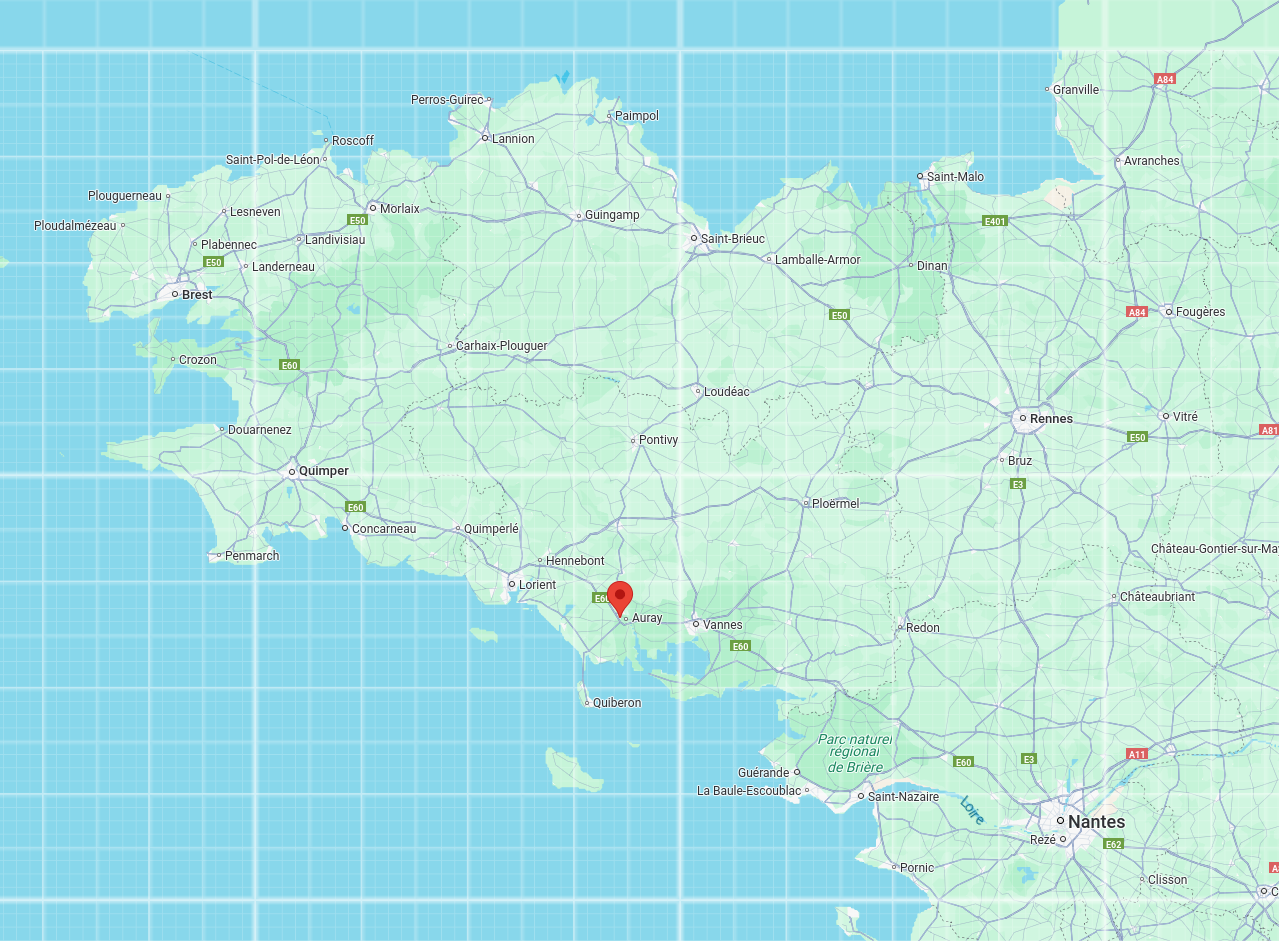
\includegraphics[width=0.4\textwidth]{../img/localisation.png}}
  				\end{overpic}
  				\vspace{0.3cm}
				\caption{
				  	\centering			
  					\href{https://maps.app.goo.gl/11j9ZHKrL6TVrdYB6}{\underline{32 rue du Danemark, Brech 56400}}.\\
  					\textit{Source : Google Maps.}
				}
  				\label{fig:localisation}
  			\end{figure}
  		\end{minipage}
	\end{center}
	\vfill
\end{frame}

\begin{frame}{Qui est E-declic ?}
	\logoEdeclic
	
	\begin{beamercolorbox}[wd=\paperwidth,ht=1.5em,dp=0.5em,leftskip=0.5cm]{section in head/foot}
  		\large \textbf{Bsoins et objectifs}
	\end{beamercolorbox}
	\vspace{0.5em}
	\begin{center}
  		\begin{minipage}{0.9\textwidth}
			\textbf{Besoins}
			\begin{itemize}
				\item Répondre aux demandes en développement web.
				\item Créer des outils numériques sur mesure.
			\end{itemize}
	
			\pause	
	
			\textbf{Objectifs}
			\begin{itemize}
				\item Assurer la qualité et la fiabilité des services.
				\item Maintenir une rentabilité positive.
				\item Créer des sites web écoresponsables.
			\end{itemize}
  		\end{minipage}
	\end{center}
	\vfill
\end{frame}

\begin{frame}{Qui est E-declic ?}
	\logoEdeclic
	
	\begin{beamercolorbox}[wd=\paperwidth,ht=1.5em,dp=0.5em,leftskip=0.5cm]{section in head/foot}
  		\large \textbf{Moyen de coordination et de direction}
	\end{beamercolorbox}
	\vspace{0.5em}
	\begin{center}
  		\begin{minipage}{0.9\textwidth}
			\begin{figure}[t]
  				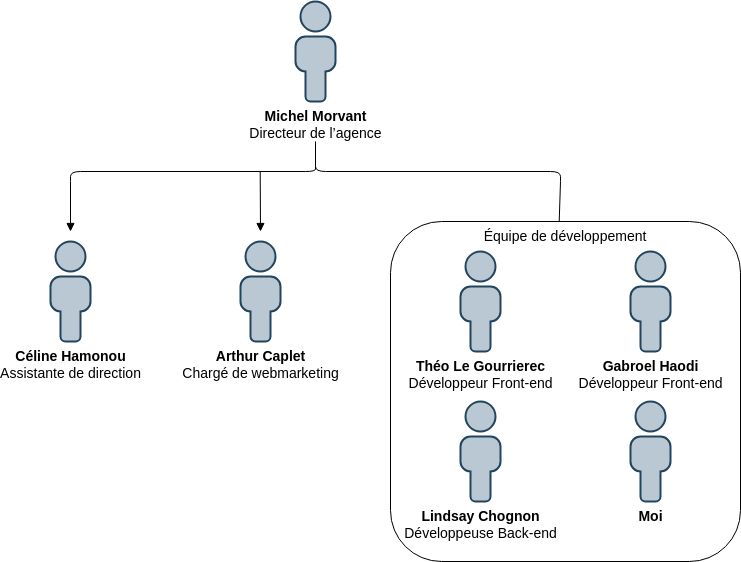
\includegraphics[height=5.5cm]{../img/coordination.png}
  				\caption{
					\centering    					
    					\href{https://www.e-declic.com/agence-web/equipe/}{\underline{Organigramme de l'entreprise}}.\\
    					\textit{Source : Mattéo Kervadec}
  				}
  				\label{fig:coordination}
  			\end{figure}
  		\end{minipage}
	\end{center}
	\vfill
\end{frame}

\planSlide{2}

% === SUJET DE STAGE ===
\begin{frame}[label=sujet]{Les missions et objectifs du stage}

	\begin{beamercolorbox}[wd=\paperwidth,ht=1.5em,dp=0.5em,leftskip=0.5cm]{section in head/foot}
  		\large \textbf{Sujet de stage}
	\end{beamercolorbox}
	\vspace{0.2em}
	
	\begin{center}
  		\begin{minipage}{0.9\textwidth}				

    		\hspace{0.5cm} \small Le stage de \textbf{développement d'applications web} se concentrera sur la création, l'amélioration, et la maintenance d'applications web \textbf{interactives}, \textbf{responsive}, et \textbf{sécurisées}. Le stagiaire participera activement au développement de fonctionnalités côté client (\textbf{frontend}) et côté serveur (\textbf{backend}), selon les besoins du projet, tout en \textbf{respectant les bonnes pratiques} en matière de \textbf{code}, de \textbf{performance} et de \textbf{sécurité}. Le stagiaire \textbf{sera impliqué} dans plusieurs étapes du cycle de \textbf{développement} d'une application web, de la \textbf{planification} et \textbf{conception} à l'implémentation et aux \textbf{tests}. Le projet pourra inclure la \textbf{création de nouvelles applications}, l'\textbf{ajout de fonctionnalités} à des systèmes existants, ou encore la \textbf{refonte d'applications} pour améliorer leur performance et leur expérience utilisateur.
				
  		\end{minipage}
	\end{center}
	\vfill
\end{frame}

\begin{frame}{Les missions et objectifs du stage}

	\begin{beamercolorbox}[wd=\paperwidth,ht=1.5em,dp=0.5em,leftskip=0.5cm]{section in head/foot}
  		\large \textbf{Sujet de stage}
	\end{beamercolorbox}
	\vspace{0.2em}
	
	\begin{center}
  		\begin{minipage}{1\textwidth}				

    			\faLaptopCode\ \textbf{Développement web full-stack :}
      		\begin{itemize}
        			\item Frontend \& Backend
        			\item Interactives \& Responsives
      		\end{itemize}

			\pause

    			\vspace{0.5em}
    			\faCheckCircle\ \textbf{Bonnes pratiques :}
      		\begin{itemize}
        			\item Programmation, performance et sécurité
      		\end{itemize}

			\pause

    			\vspace{0.5em}
    			\faProjectDiagram\ \textbf{Cycle de développement :}
      		\begin{itemize}
        			\item Planification → Conception → Implémentation → Tests
      		\end{itemize}

			\pause

    			\vspace{0.5em}
    			\faTasks\ \textbf{Missions possibles :}
      		\begin{itemize}
        			\item Nouvelles apps, fonctionnalités, refonte
      		\end{itemize}
  		\end{minipage}
	\end{center}
	\vfill
\end{frame}

\begin{frame}{Les missions et objectifs du stage}

	Comment répondre aux besoins spécifiques de réservation en ligne de produits pour des hébergements touristiques via une application web, et permettre à l’agence E-declic d’élargir son offre de services ?
			
	\begin{center}
  		\begin{minipage}{0.9\textwidth}
  			\vspace{10cm}
  		\end{minipage}
	\end{center}
	\vfill
\end{frame}

\begin{frame}{Les missions et objectifs du stage}

	Comment répondre aux besoins spécifiques de réservation en ligne de produits pour des hébergements touristiques via une application web, et permettre à l’agence E-declic d’élargir son offre de services ?
			
	\begin{center}
  		\begin{minipage}{0.9\textwidth}
			\begin{beamercolorbox}[wd=\paperwidth,ht=1.5em,dp=0.5em,leftskip=0.5cm]{section in head/foot}
  				\large \textbf{Missions confiées} - \href{https://github.com/Matteo-K/Soutenance_E-delic/blob/main/pdf/cc-painspizzas-camping.pdf}{\underline{(Lien du pdf sur github)}}
			\end{beamercolorbox}
			\begin{itemize}
				\item<1-> Gestion d'hébergements
				\item<1-> Gestion d'utilisateur
				\item<2-> Gestion du E-commerce
				\begin{itemize}
					\item Gestion de produit
					\item Gestion du panier
					\item Gestion du paiement
					\item \textbf{Gestion de la disponibilité des produits}
				\end{itemize}
				\item<3-> Gestion de l'administration
			\end{itemize}
  		\end{minipage}
  		\vspace{1cm}
	\end{center}
	\vfill
\end{frame}

\begin{frame}{Les missions et objectifs du stage}

	Comment répondre aux besoins spécifiques de réservation en ligne de produits pour des hébergements touristiques via une application web, et permettre à l’agence E-declic d’élargir son offre de services ?
			
	\begin{center}
  		\begin{minipage}{0.9\textwidth}
			\begin{beamercolorbox}[wd=\paperwidth,ht=1.5em,dp=0.5em,leftskip=0.5cm]{section in head/foot}
  				\large \textbf{Principales difficultés attendues}
			\end{beamercolorbox}
			
			\begin{itemize}
				\item<1-> Gestion multi-utilisateur → multi-rôles
				\item<2-> Gestion de la disponibilité des produits
				\begin{itemize}
					\item Gestion du produit
					\item Gestoin du panier
					\item Gestion des commandes
					\item Gestion de l'historique
				\end{itemize}
				\item<3-> Intégration du paiement via stripe
			\end{itemize}
  			\vspace{1cm}
  		\end{minipage}
	\end{center}
	\vfill
\end{frame}

\planSlide{3}

% === ENVIRONNEMENT ===
\begin{frame}[label=environnement]{Environnement de travail}
	\begin{beamercolorbox}[wd=\paperwidth,ht=1.5em,dp=0.5em,leftskip=0.5cm]{section in head/foot}
  		\large \textbf{Outils utilisés}
	\end{beamercolorbox}
	\vspace{0.5em}
	\begin{center}
  		\begin{minipage}{0.9\textwidth}
  			\begin{columns}[T, onlytextwidth]
        			\column{0.48\textwidth}
        				
        				% Looping
        				\begin{minipage}[t][2cm][t]{\linewidth}
        					\raggedright
         				
\includegraphics[width=1.35cm, height=0.75cm, keepaspectratio]{../img/logo_looping.png} 
         				\hspace{0.1cm} \textbf{Looping} \\ 
         				Gestionnaire de modélisation de base de données
          		  	\end{minipage}
          			\vspace{0.7em}
          			\pause
          			
          			% Figma
        				\begin{minipage}[t][2cm][t]{\linewidth}
        					\raggedright
          				
\includegraphics[height=0.75cm]{../img/logo_figma.png}
          				\hspace{0.95cm} \textbf{Figma} \\
          				Conception des maquettes et prototypes
          			\end{minipage}
          			\vspace{0.7em}
          			\pause
          		
          			% Windsurf	
          			\begin{minipage}[t][2cm][t]{\linewidth}
          				\raggedright
          				
\includegraphics[width=0.75cm, height=0.75cm]{../img/logo_windsurf.png}
          				\hspace{0.6cm} \textbf{Windsurf} \\ 
          				Editeur de texte
          			\end{minipage}
          			\pause
          			
        			\column{0.48\textwidth}
        			
        				% Postman
        				\begin{minipage}[t][2cm][t]{\linewidth}
        					\raggedright
          				
\includegraphics[width=0.75cm, height=0.75cm]{../img/logo_postman.png}
          				\hspace{0.6cm} \textbf{Postman} \\
          				Tester et envoyer des requêtes serveurs (API)
          			\end{minipage}
          			\vspace{0.7em}
          			\pause
          			
          			% Github
          			\begin{minipage}[t][2cm][t]{\linewidth}
          				\raggedright
          				
\includegraphics[width=0.75cm, height=0.75cm]{../img/logo_github.png}
          				\hspace{0.6cm} \textbf{Github} \\
          				Gestion du versioning et partage de fichiers
          			\end{minipage}
          			\vspace{0.7em}
          			\pause
          			
          			% Slack
          			\begin{minipage}[t][2cm][t]{\linewidth}
          				\raggedright
          				
\includegraphics[width=0.75cm, height=0.75cm]{../img/logo_slack.png}
          				\hspace{0.6cm} \textbf{Slack} \\
          				Messagerie instantanée
          			\end{minipage}

      		\end{columns}
  		\end{minipage}
	\end{center}
	\vfill
\end{frame}

\begin{frame}{Environnement de travail}
	\begin{beamercolorbox}[wd=\paperwidth,ht=1.5em,dp=0.5em,leftskip=0.5cm]{section in head/foot}
  		\large \textbf{Langages utilisés}
	\end{beamercolorbox}
	\vspace{0.5em}
	\begin{center}
		\begin{minipage}{0.9\textwidth}
  			\begin{columns}[T, onlytextwidth]
    				\column{0.48\textwidth}
    
    					\vspace{2.5em}
      				% Symfony
      				\begin{minipage}[t][2cm][t]{\linewidth}
        					\raggedright
        					
\includegraphics[height=0.75cm]{../img/logo_symfony.png}
        					\hspace{0.6cm} \textbf{Symfony} \\
        					Framework PHP pour l'architecture backend
      				\end{minipage}
      				\vspace{0.7em}
          			\pause
      
      				% Twig
      				\begin{minipage}[t][2cm][t]{\linewidth}
        					\raggedright
        					
\includegraphics[height=0.75cm]{../img/logo_twig.png}
        					\hspace{0.6cm} \textbf{Twig} \\
        					Générateur de vues Html pour Symfony
      				\end{minipage}
          			\pause

    				\column{0.48\textwidth}
    
      				% Turbo / Stimulus
      				\begin{minipage}[t][2cm][t]{\linewidth}
        					\raggedright
        					\textbf{Turbo/Stimulus} \\
        					Interaction frontend et mises à jour dynamiques
      				\end{minipage}
      				\vspace{0.7em}
          			\pause
      
      				% Twig Components
      				\begin{minipage}[t][2cm][t]{\linewidth}
        					\raggedright
        					\textbf{Twig Components} \\
        					Représentation réutilisable des éléments d'interface
      				\end{minipage}
      				\vspace{0.7em}
          			\pause
      
      				% Autocomplete
      				\begin{minipage}[t][2cm][t]{\linewidth}
        					\raggedright
        					\textbf{Autocomplete} \\
        					Champ de saisie avec suggestions dynamiques
      				\end{minipage}
      
  			\end{columns}
		\end{minipage}
	\end{center}
	\vfill
\end{frame}

\begin{frame}[label=env]{Environnement de travail}
    \begin{beamercolorbox}[wd=\paperwidth,ht=1.5em,dp=0.5em,leftskip=0.5cm]{section in head/foot}
        \large \textbf{Moyens d'organisation du projet}
    \end{beamercolorbox}
    \vspace{0.5em}
    \begin{center}
\begin{minipage}{0.9\textwidth}
    \begin{itemize}
        \item<1-> \textbf{Méthode de travail :} gestion souple, sans cadre agile
        \item<2-> \textbf{Réunion :} point hebdomadaire (lundi 10h)
        \item<3-> \textbf{Suivi des tâches :} carnet de fonctionnalités
        \item<4-> \textbf{Gestion des incidents :} journal des problèmes et solutions
        \item<5-> \textbf{Communication :} échanges quotidiens et à distance via Slack
    \end{itemize}
\end{minipage}

    \end{center}
    \vfill
\end{frame}

\begin{frame}[label=env]{Environnement de travail}  
	\begin{beamercolorbox}[wd=\paperwidth,ht=1.5em,dp=0.5em,leftskip=0.5cm]{section in head/foot}
  		\large \textbf{Planning Gantt et organisation personnelle}
	\end{beamercolorbox}
	\vspace{0.5em}
	\begin{center}
		\begin{minipage}{0.9\textwidth}
			\begin{figure}[t]
  				\centering
  				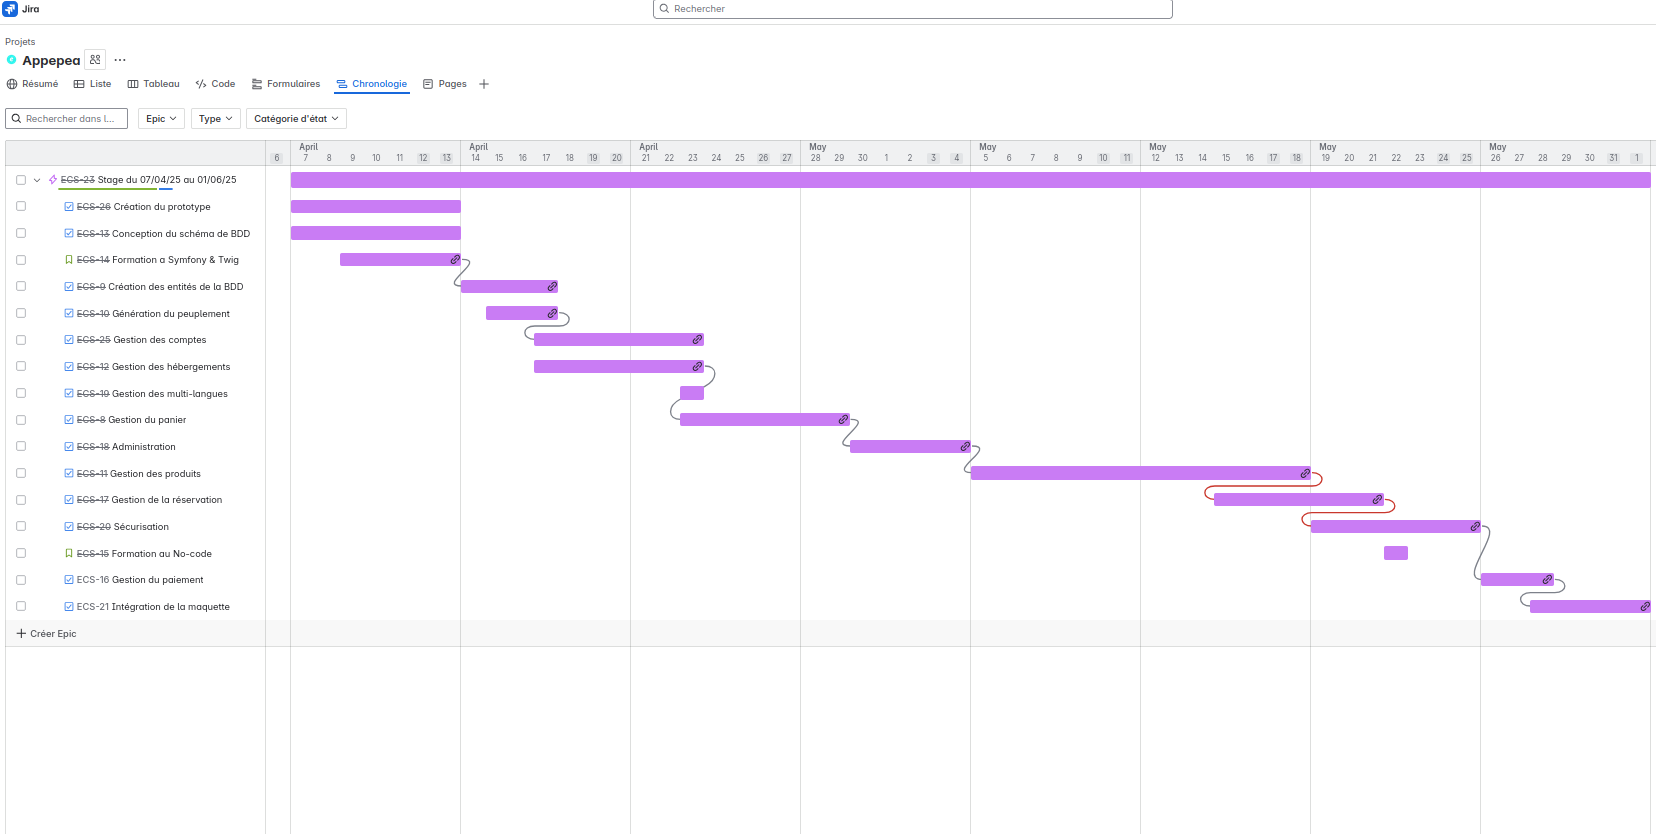
\includegraphics[height=5cm]{../img/gantt.png}
  				\caption{
    					\href{https://etudiant-team-z8ihahyp.atlassian.net/jira/software/projects/ECS/boards/1/timeline?timeline=WEEKS}{\underline{Diagramme Gantt}}.\\
    					\textit{Source : Mattéo Kervadec}
  				}
  				\label{fig:gantt}
			\end{figure}
		\end{minipage}
	\end{center}
	\vfill
\end{frame}

\planSlide{4}

% === REALISATIONS ===
\begin{frame}[label=realisation]{Solutions apportées aux projets}
	\begin{beamercolorbox}[wd=\paperwidth,ht=1.5em,dp=0.5em,leftskip=0.5cm]{section in head/foot}
  		\large \textbf{Réalisation 1 :} \normalsize Conception et modélisation de l'application
	\end{beamercolorbox}
	\vspace{0.5em}

	\begin{center}
  		\only<1-4> {
  			\begin{minipage}{0.9\textwidth}
  				\textbf{Situation :} Le projet manquait d’une structure claire pour organiser les données. \pause \\  		
  				\textbf{Tâche :} Identifier les fonctionnalités de l'application.\pause \\
  				\textbf{Action :}
  			  		\begin{itemize}
  						\item Identification des fonctionnalités
  						\item Réalisation du modèle conceptuel des données (MCD)
  						\item Création d'un \href{https://www.figma.com/design/GuunRMUtzwJjCk1OudcjYl/Pain-Pizza?node-id=0-1&p=f&t=KjBsRt1nqpntIccn-0}{\underline{prototype}} de l'application
  					\end{itemize}
  				\pause
  				
				\textbf{Résultat :} Modèle clair et globale sur les fonctionnalités facilitant le développement backend.
			\end{minipage}
		}
		\only<5> {
			\begin{figure}[t]
  				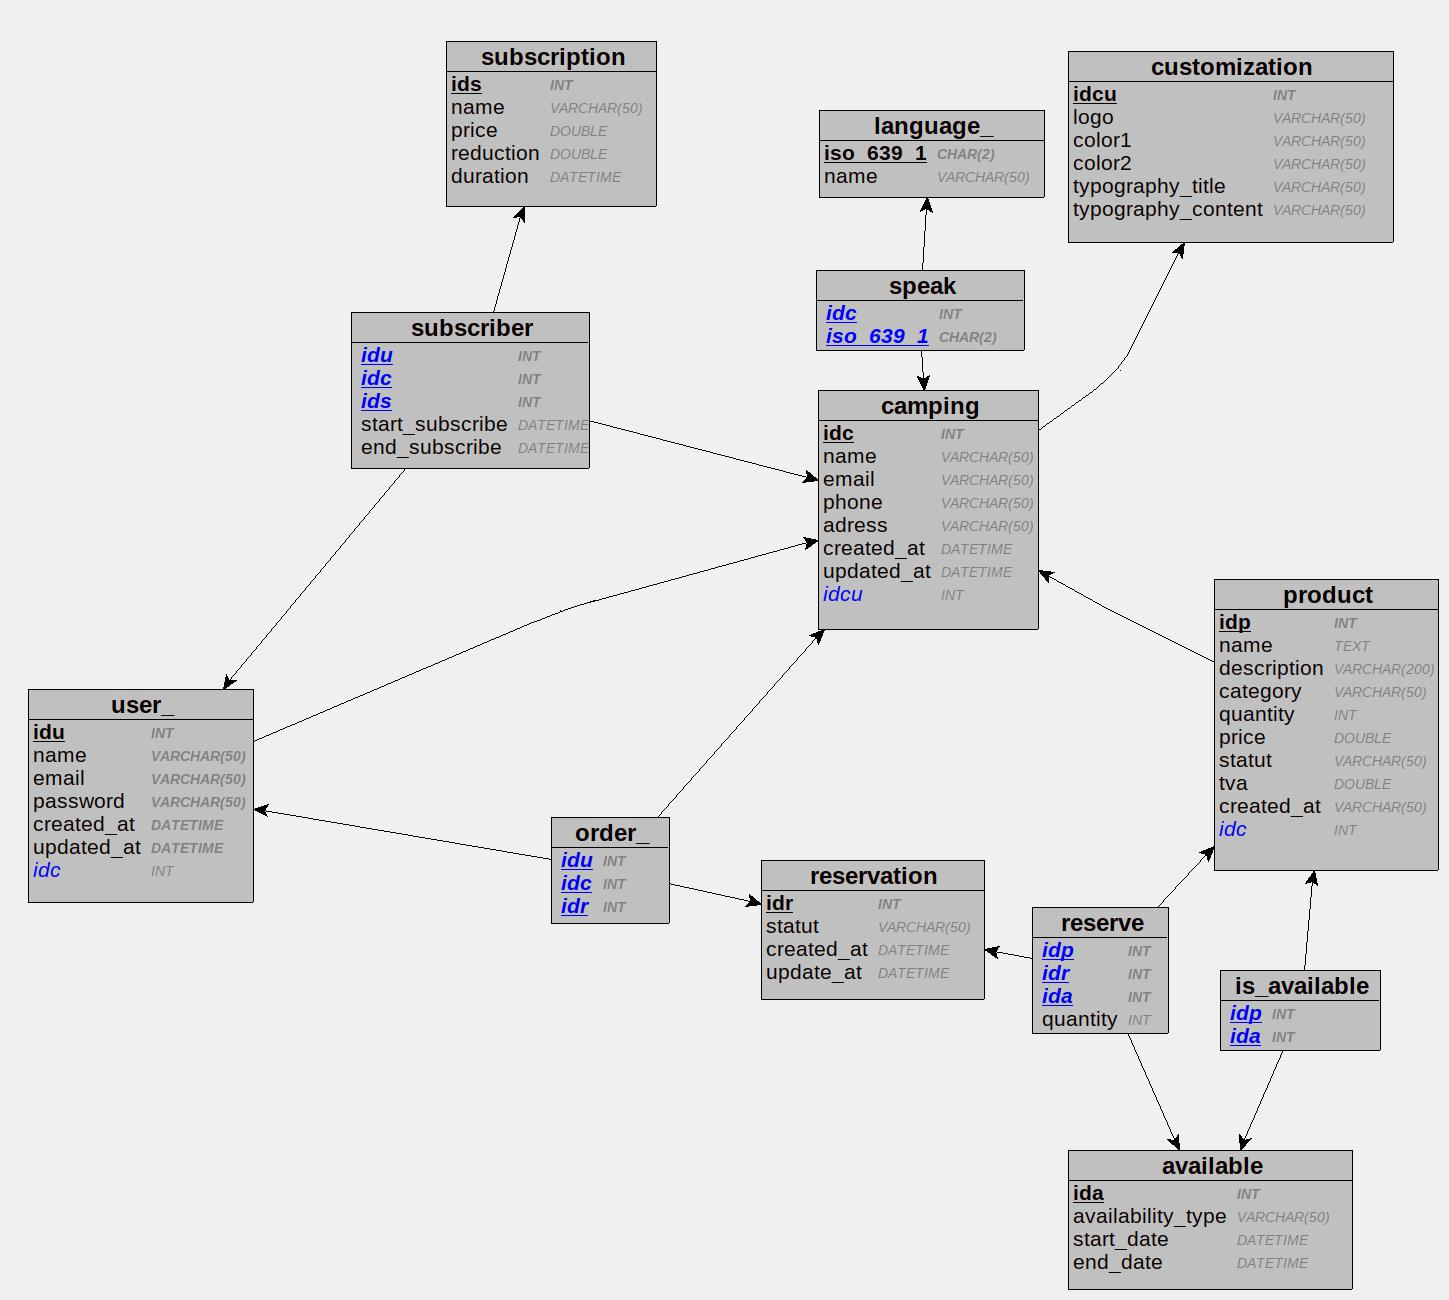
\includegraphics[height=5.5cm]{../img/conception/mcd_V1.jpg}
				\caption{	
					\centering			
  					\href{https://github.com/Matteo-K/Soutenance_E-delic/blob/main/img/conception/mcd_V1.jpg}{\underline{Modèle Conceptuel des données - version 1}}.\\
  					\textit{Source : Mattéo Kervadec}
				}
  				\label{fig:mcdV1}
  			\end{figure}
		}
		\only<6> {
			\addtocounter{figure}{1}
			\begin{figure}[t]
  				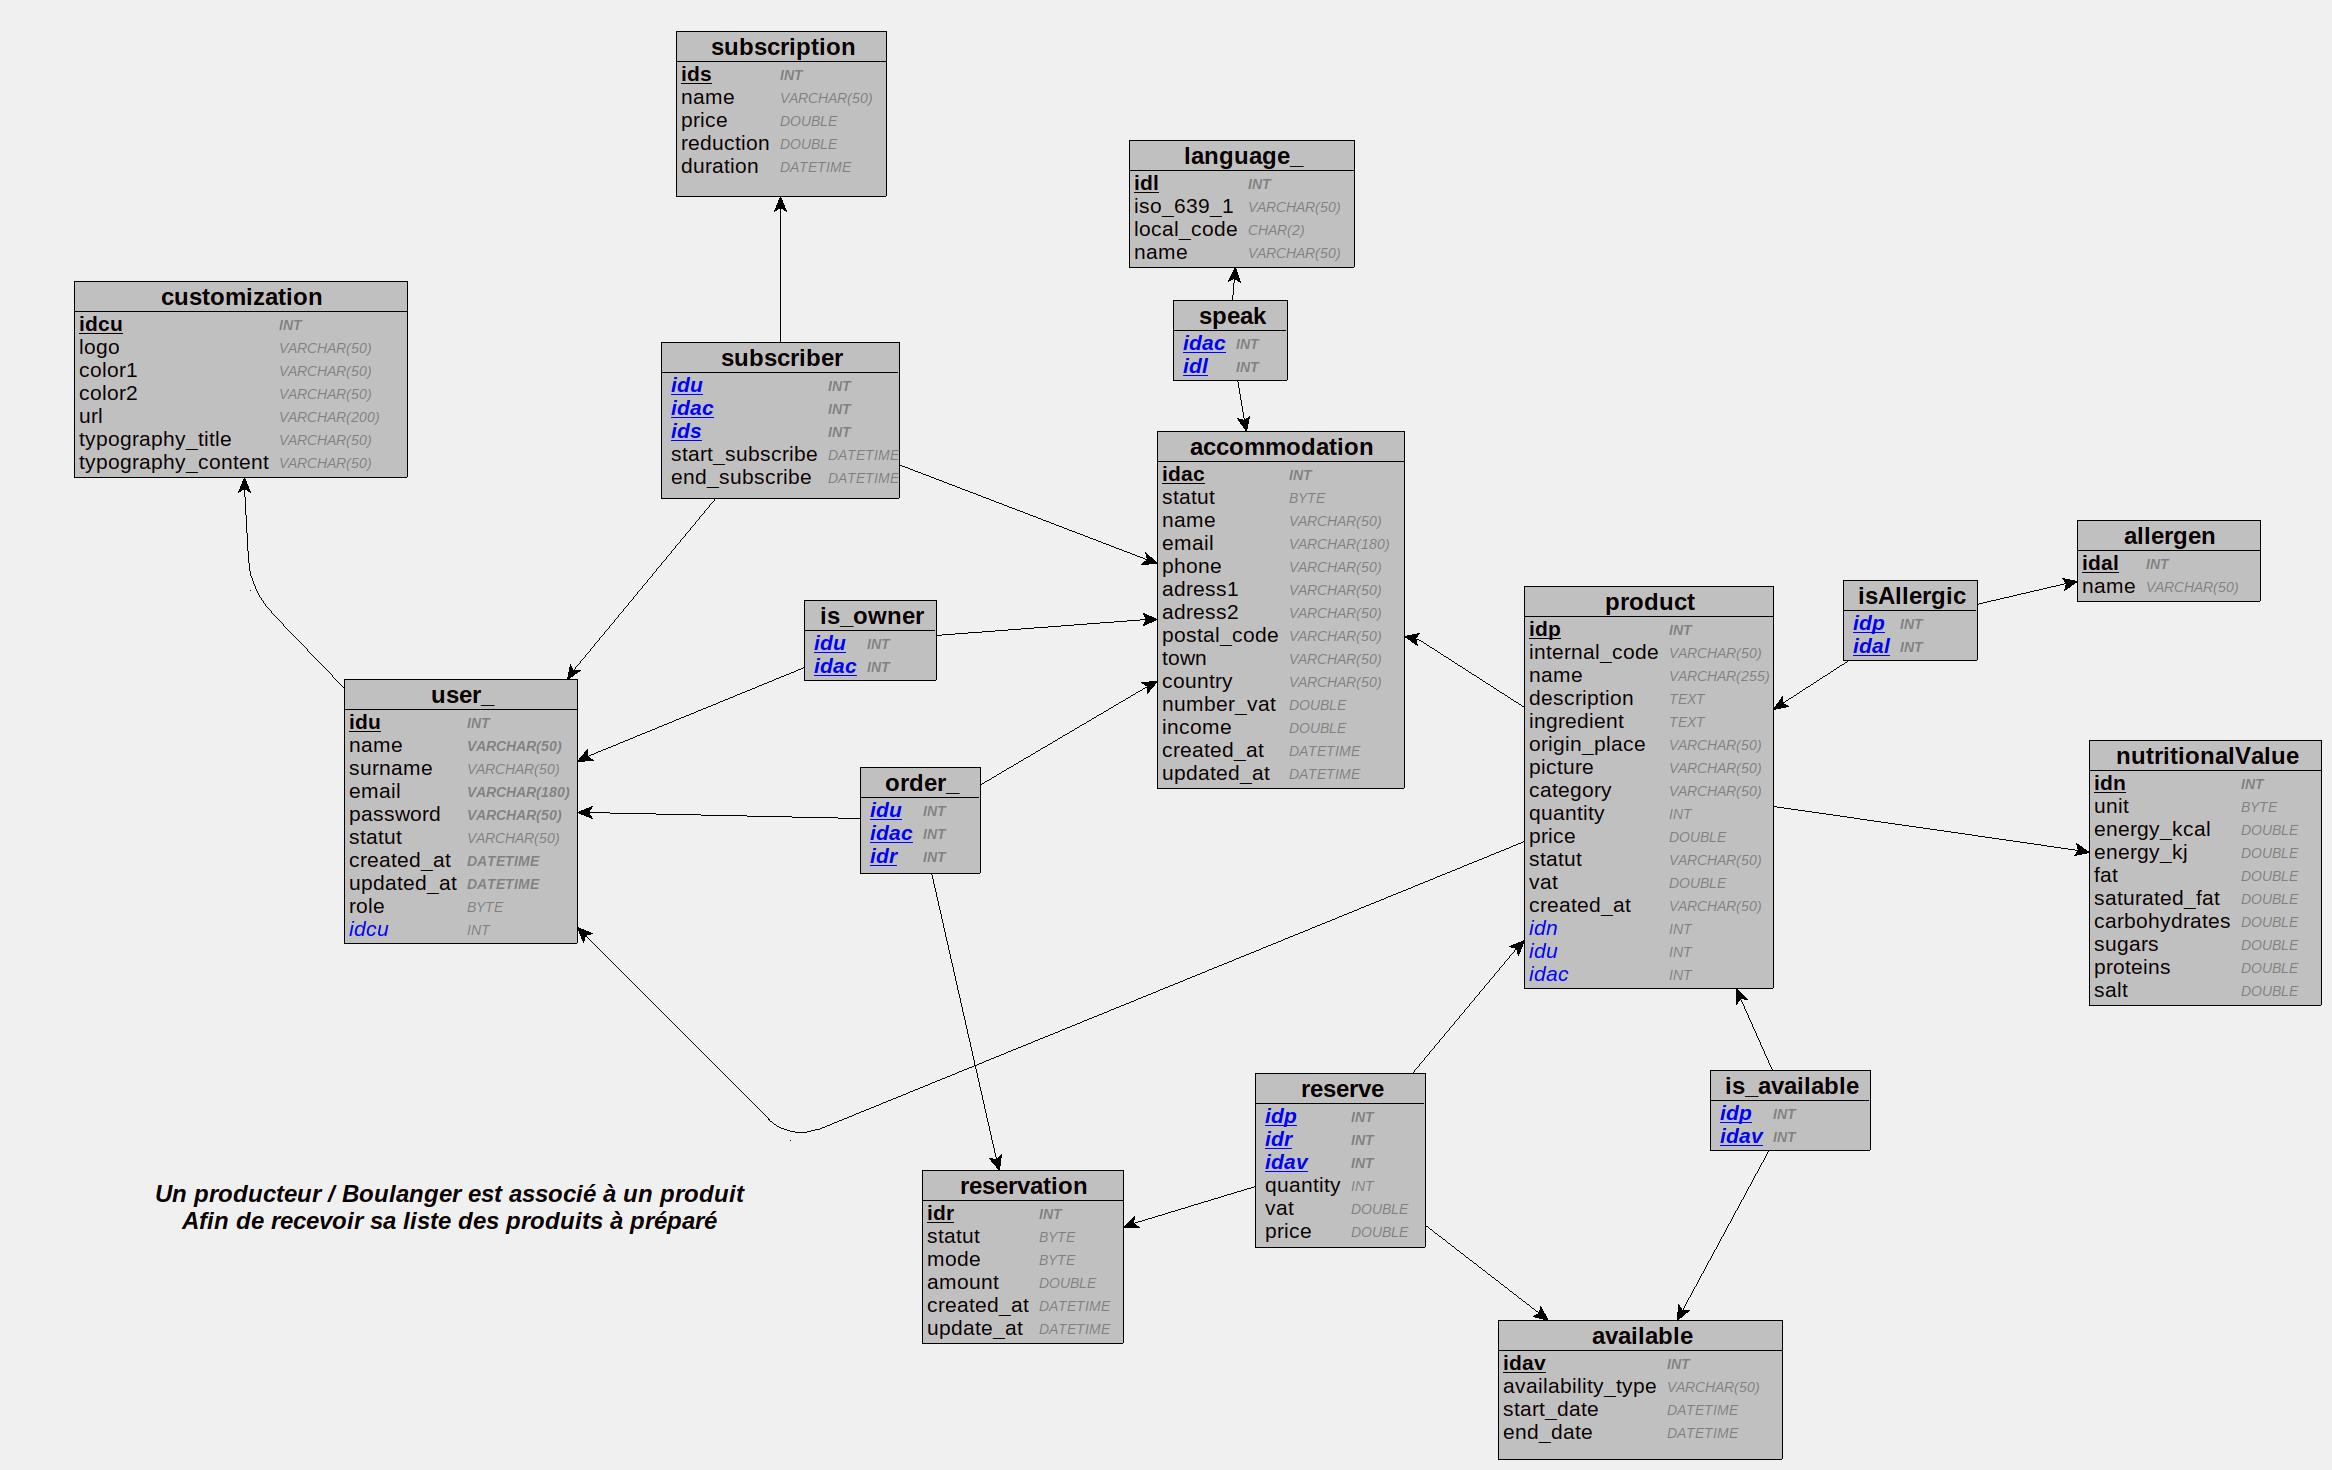
\includegraphics[height=5.5cm]{../img/conception/mcd_V2.jpg}
				\caption{	
					\centering			
  					\href{https://github.com/Matteo-K/Soutenance_E-delic/blob/main/img/conception/mcd_V2.jpg}{\underline{Modèle Conceptuel des données - version 2}}.\\
  					\textit{Source : Mattéo Kervadec}
				}
  				\label{fig:mcdV2}
  			\end{figure}
		}
		\only<7> {
			\addtocounter{figure}{2}
			\begin{figure}[t]
  				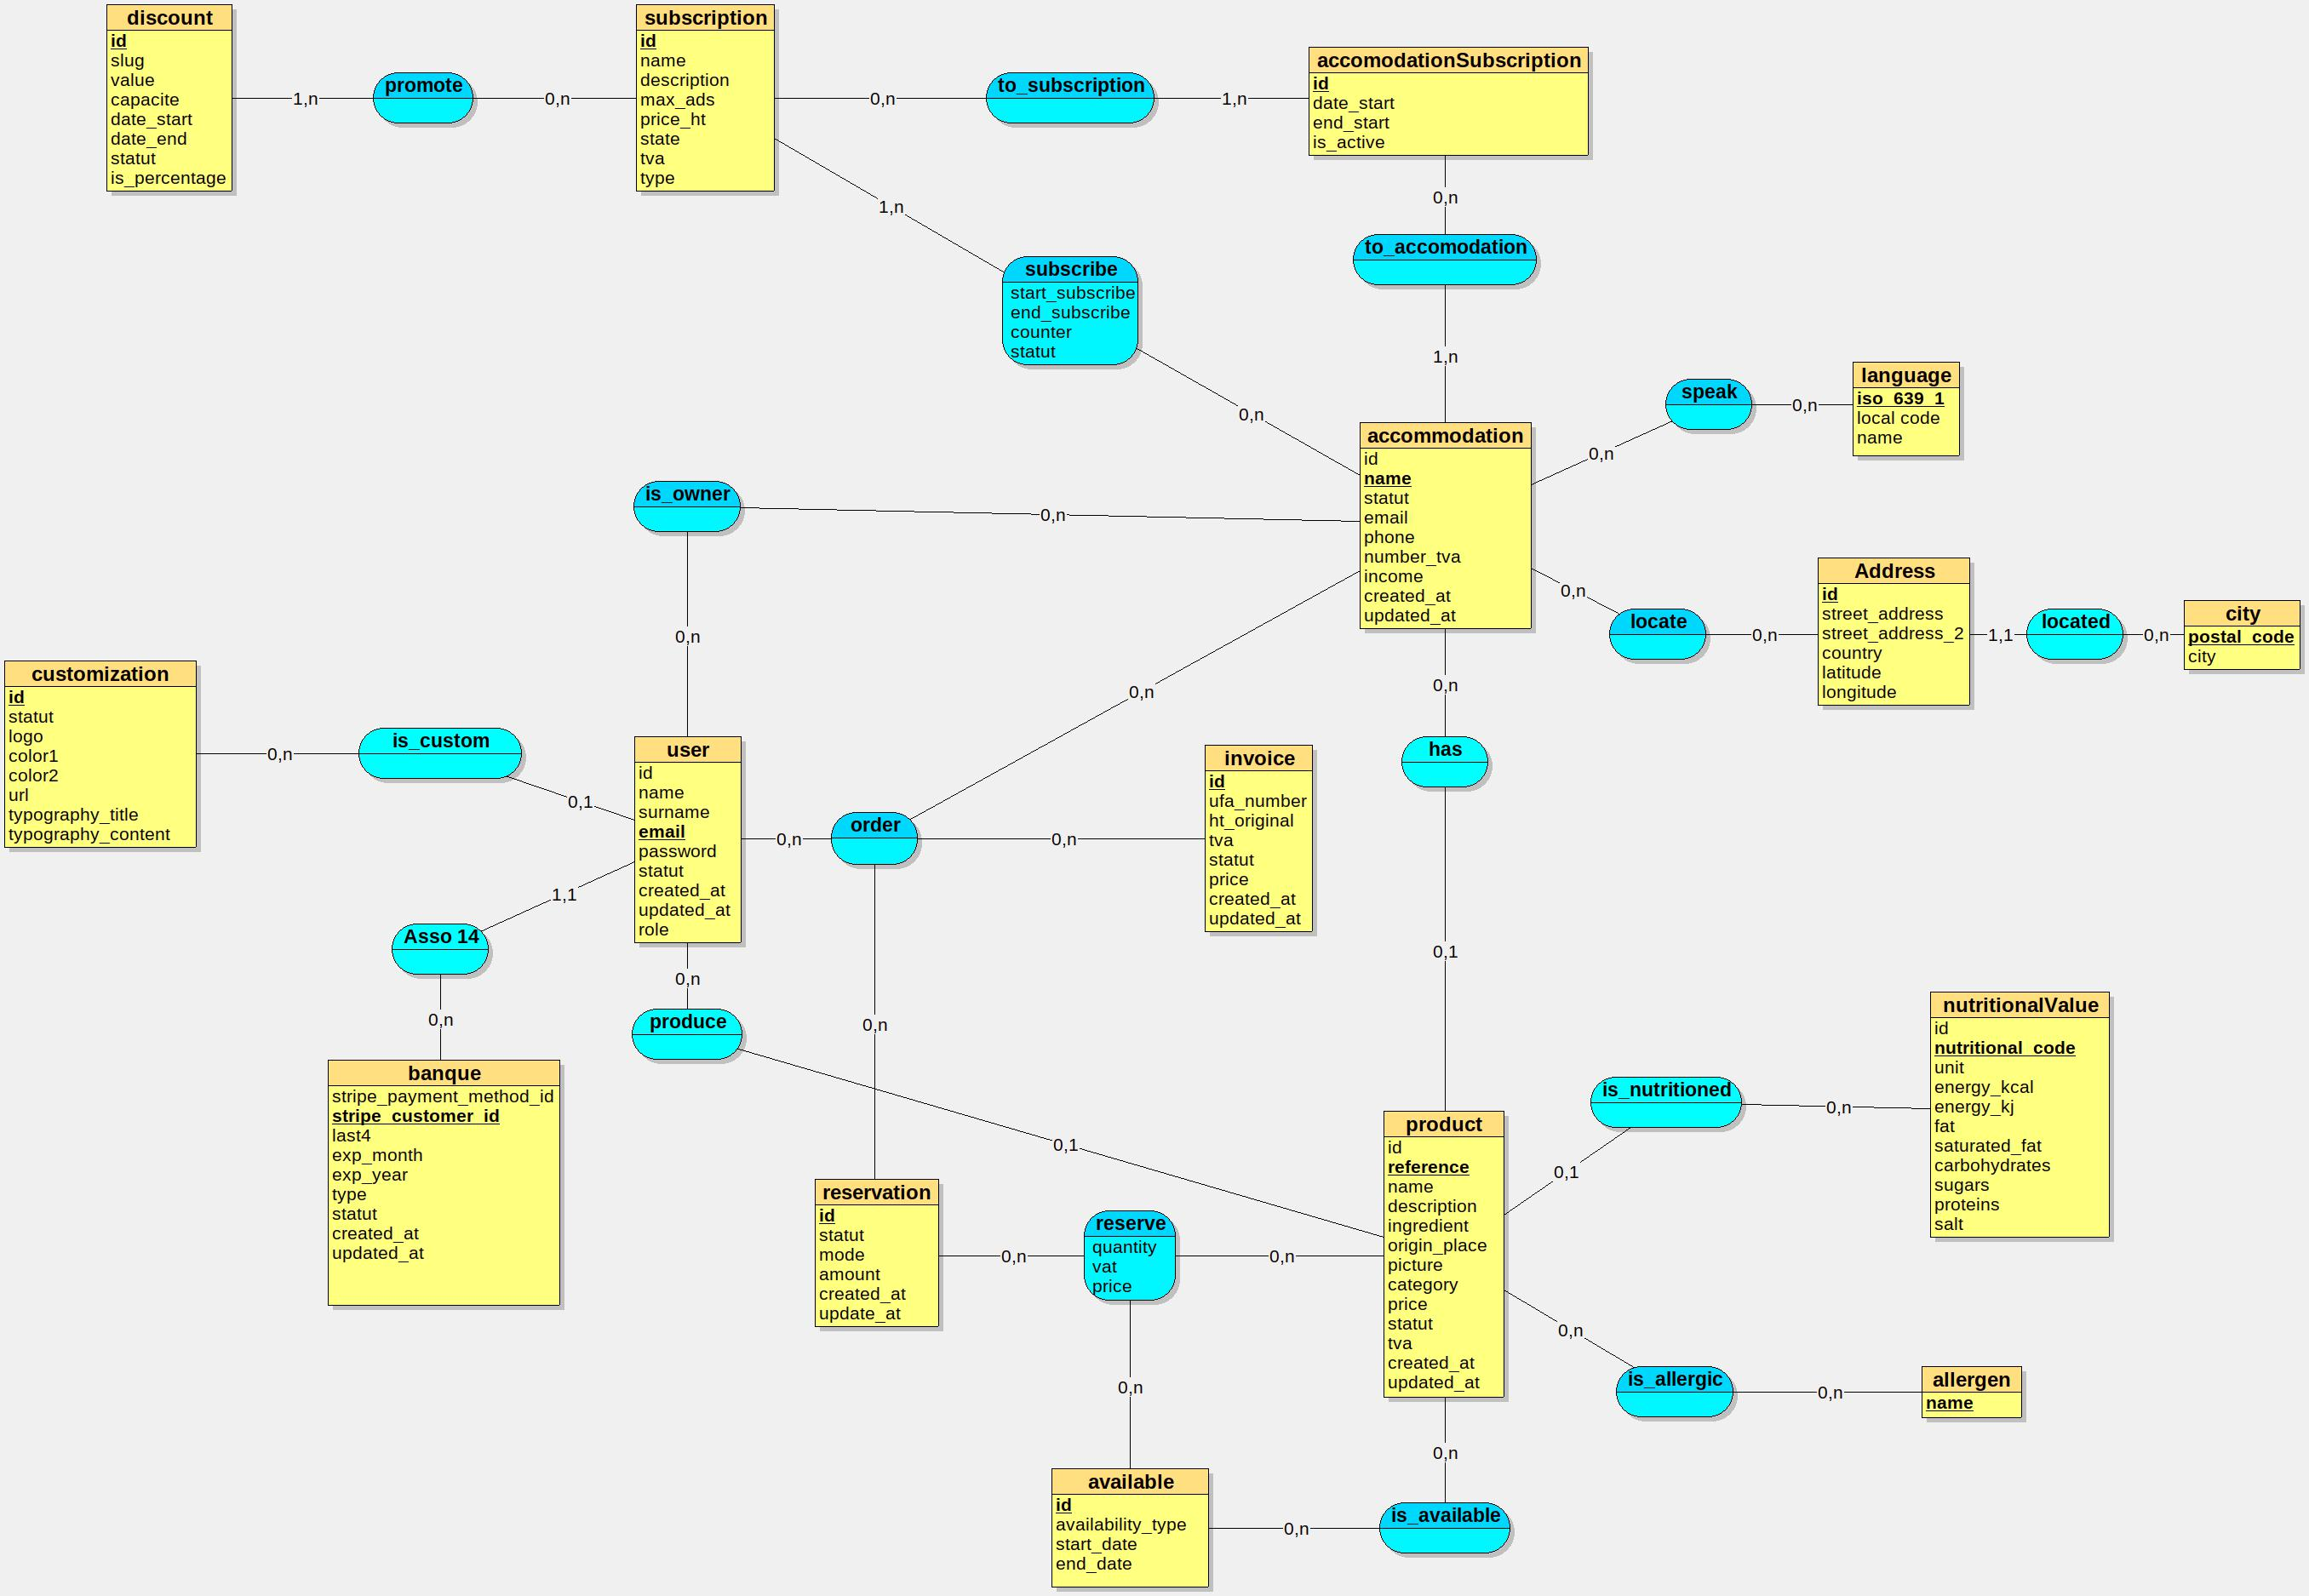
\includegraphics[height=5.5cm]{../img/conception/mcd_V3.jpg}
				\caption{	
					\centering			
  					\href{https://github.com/Matteo-K/Soutenance_E-delic/blob/main/img/conception/mcd_V3.jpg}{\underline{Modèle Conceptuel des données - version 3}}.\\
  					\textit{Source : Mattéo Kervadec}
				}
  				\label{fig:mcdV3}
  			\end{figure}
		}
		\only<8> {
			\addtocounter{figure}{3}
			\begin{figure}[t]
  				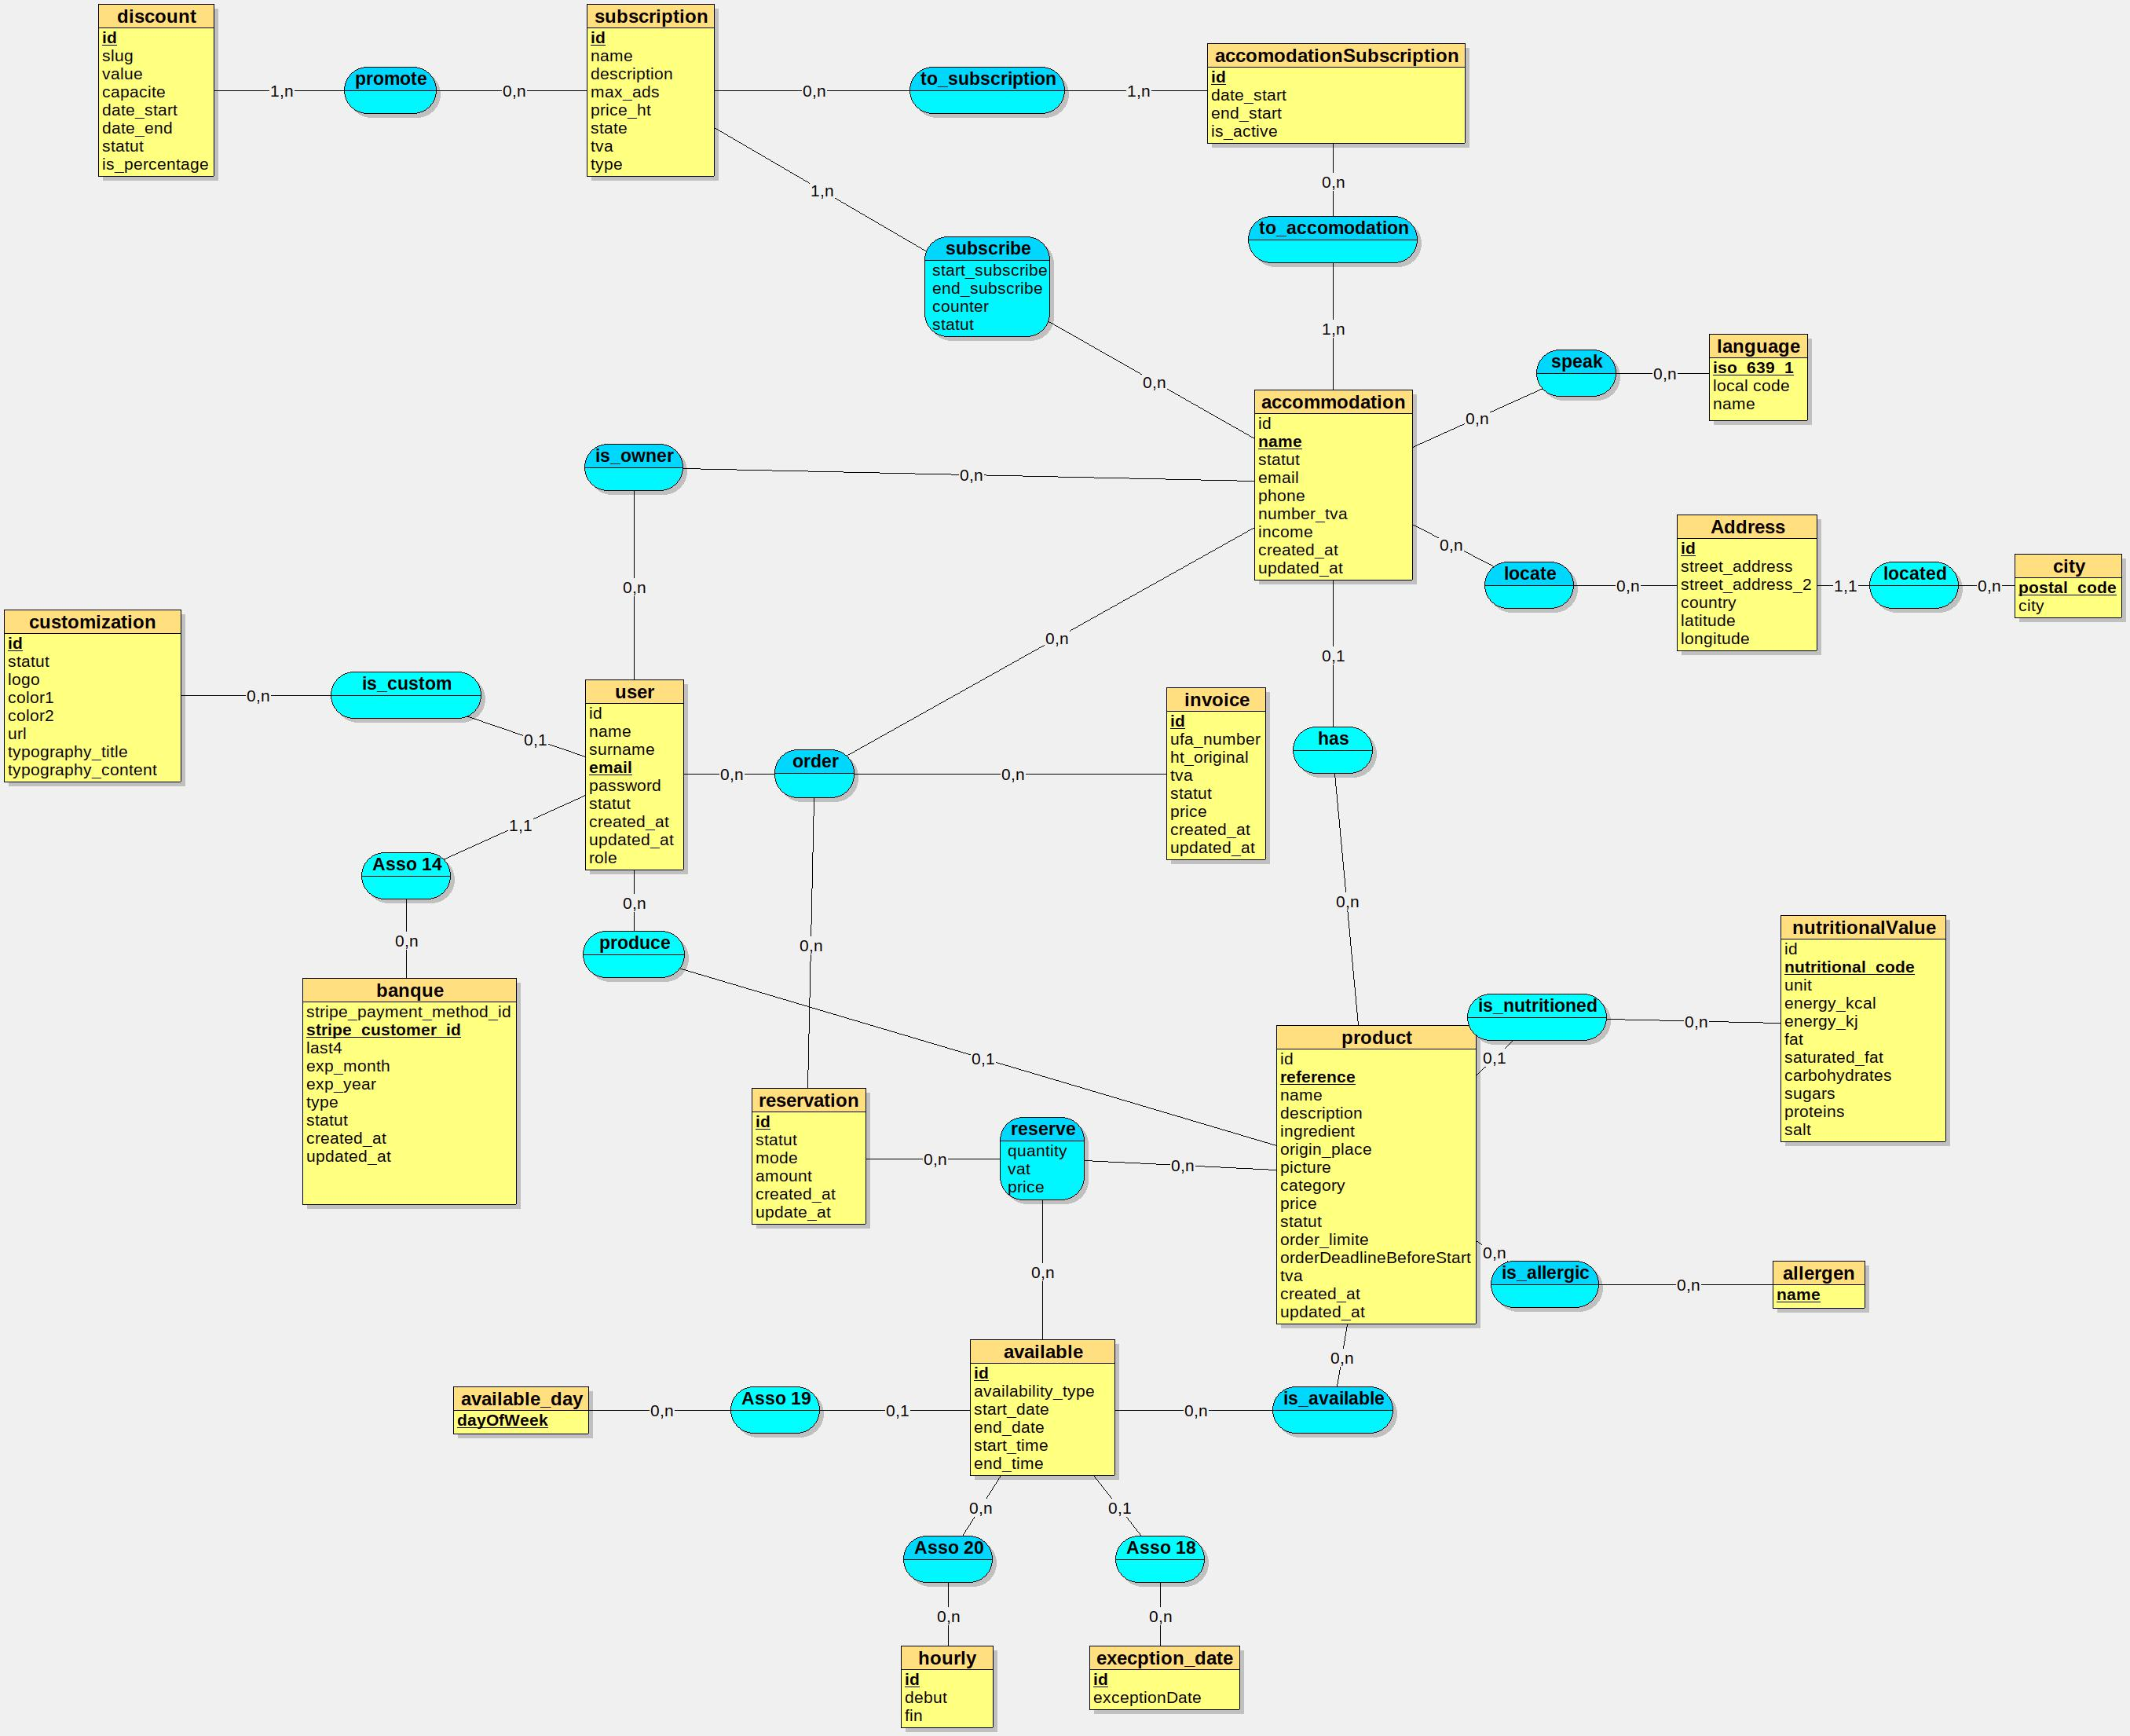
\includegraphics[height=5.5cm]{../img/conception/mcd_V4.jpg}
				\caption{	
					\centering			
  					\href{https://github.com/Matteo-K/Soutenance_E-delic/blob/main/img/conception/mcd_V4.jpg}{\underline{Modèle Conceptuel des données - version 4}}.\\
  					\textit{Source : Mattéo Kervadec}
				}
  				\label{fig:mcdV4}
  			\end{figure}
		}
		\only<9> {
			\addtocounter{figure}{4}
			\begin{figure}[t]
  				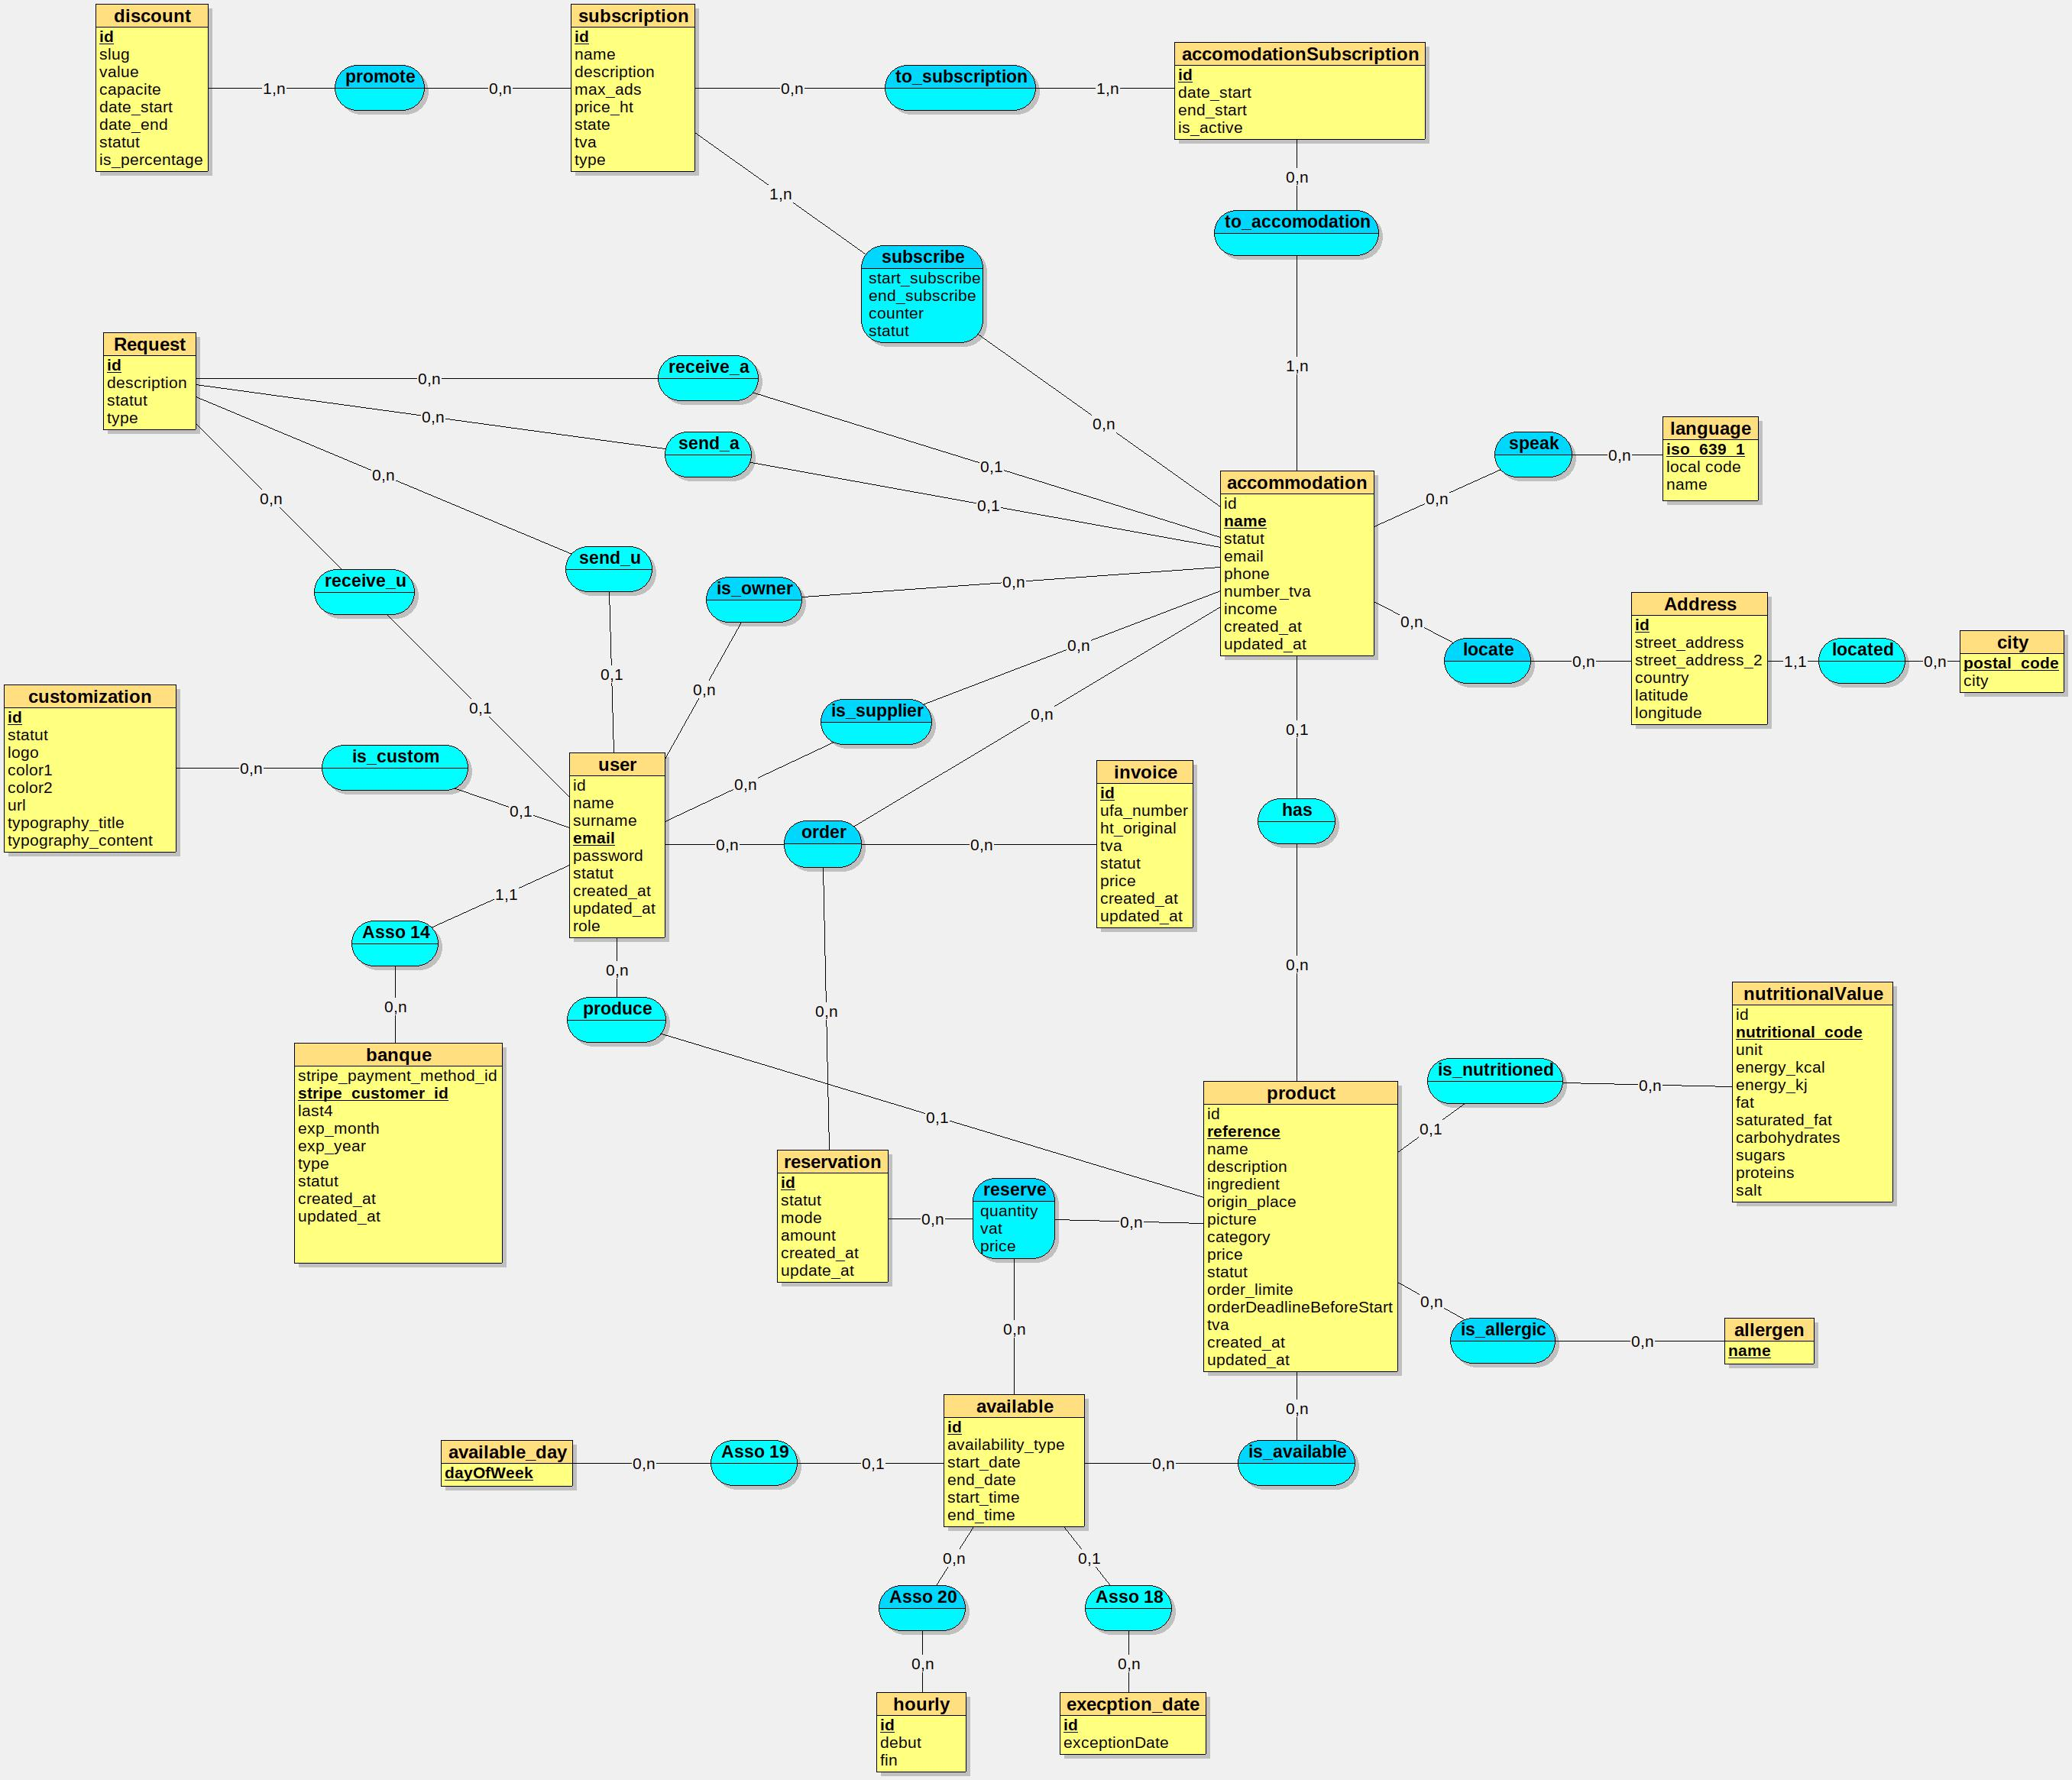
\includegraphics[height=5.5cm]{../img/conception/mcd_V5.jpg}
				\caption{	
					\centering			
  					\href{https://github.com/Matteo-K/Soutenance_E-delic/blob/main/img/conception/mcd_V5.jpg}{\underline{Modèle Conceptuel des données - version 5}}.\\
  					\textit{Source : Mattéo Kervadec}
				}
  				\label{fig:mcdV5}
  			\end{figure}
		}
	\end{center}
	\vfill
\end{frame}

\begin{frame}{Solutions apportées aux projets}
	\begin{beamercolorbox}[wd=\paperwidth,ht=1.5em,dp=0.5em,leftskip=0.5cm]{section in head/foot}
  		\large \textbf{Réalisation 2 :} \normalsize Gestion des comptes et des rôles utilisateur
	\end{beamercolorbox}
	\vspace{0.5em}
	\begin{center}
		\only<1-4> {
  			\begin{minipage}{0.9\textwidth}
  				\textbf{Situation :} Tout les utilisateurs ont un accès libre au service.\pause \\
  				\textbf{Tâche :} Gérer les rôles et les authentifications.\pause \\
  				\textbf{Action :} Mise en place de sécurités.
  				\begin{itemize}
  					\item Authentification avec JWT Tokens
  					\item Contrôle d'accès (Security \& Voter)
  					\item Usurpation des utilisateurs (Admin)
  					\end{itemize}
  				\pause

				\textbf{Résultat :}
				\begin{itemize}
					\item Multi-accès sécurisé à la plateforme
					\item Fonctionnalités adaptées selon les rôles de l'utilisateur
				\end{itemize}
	  		\end{minipage}
  		}
  		
  		\only<5> {
			\begin{figure}[t]
  				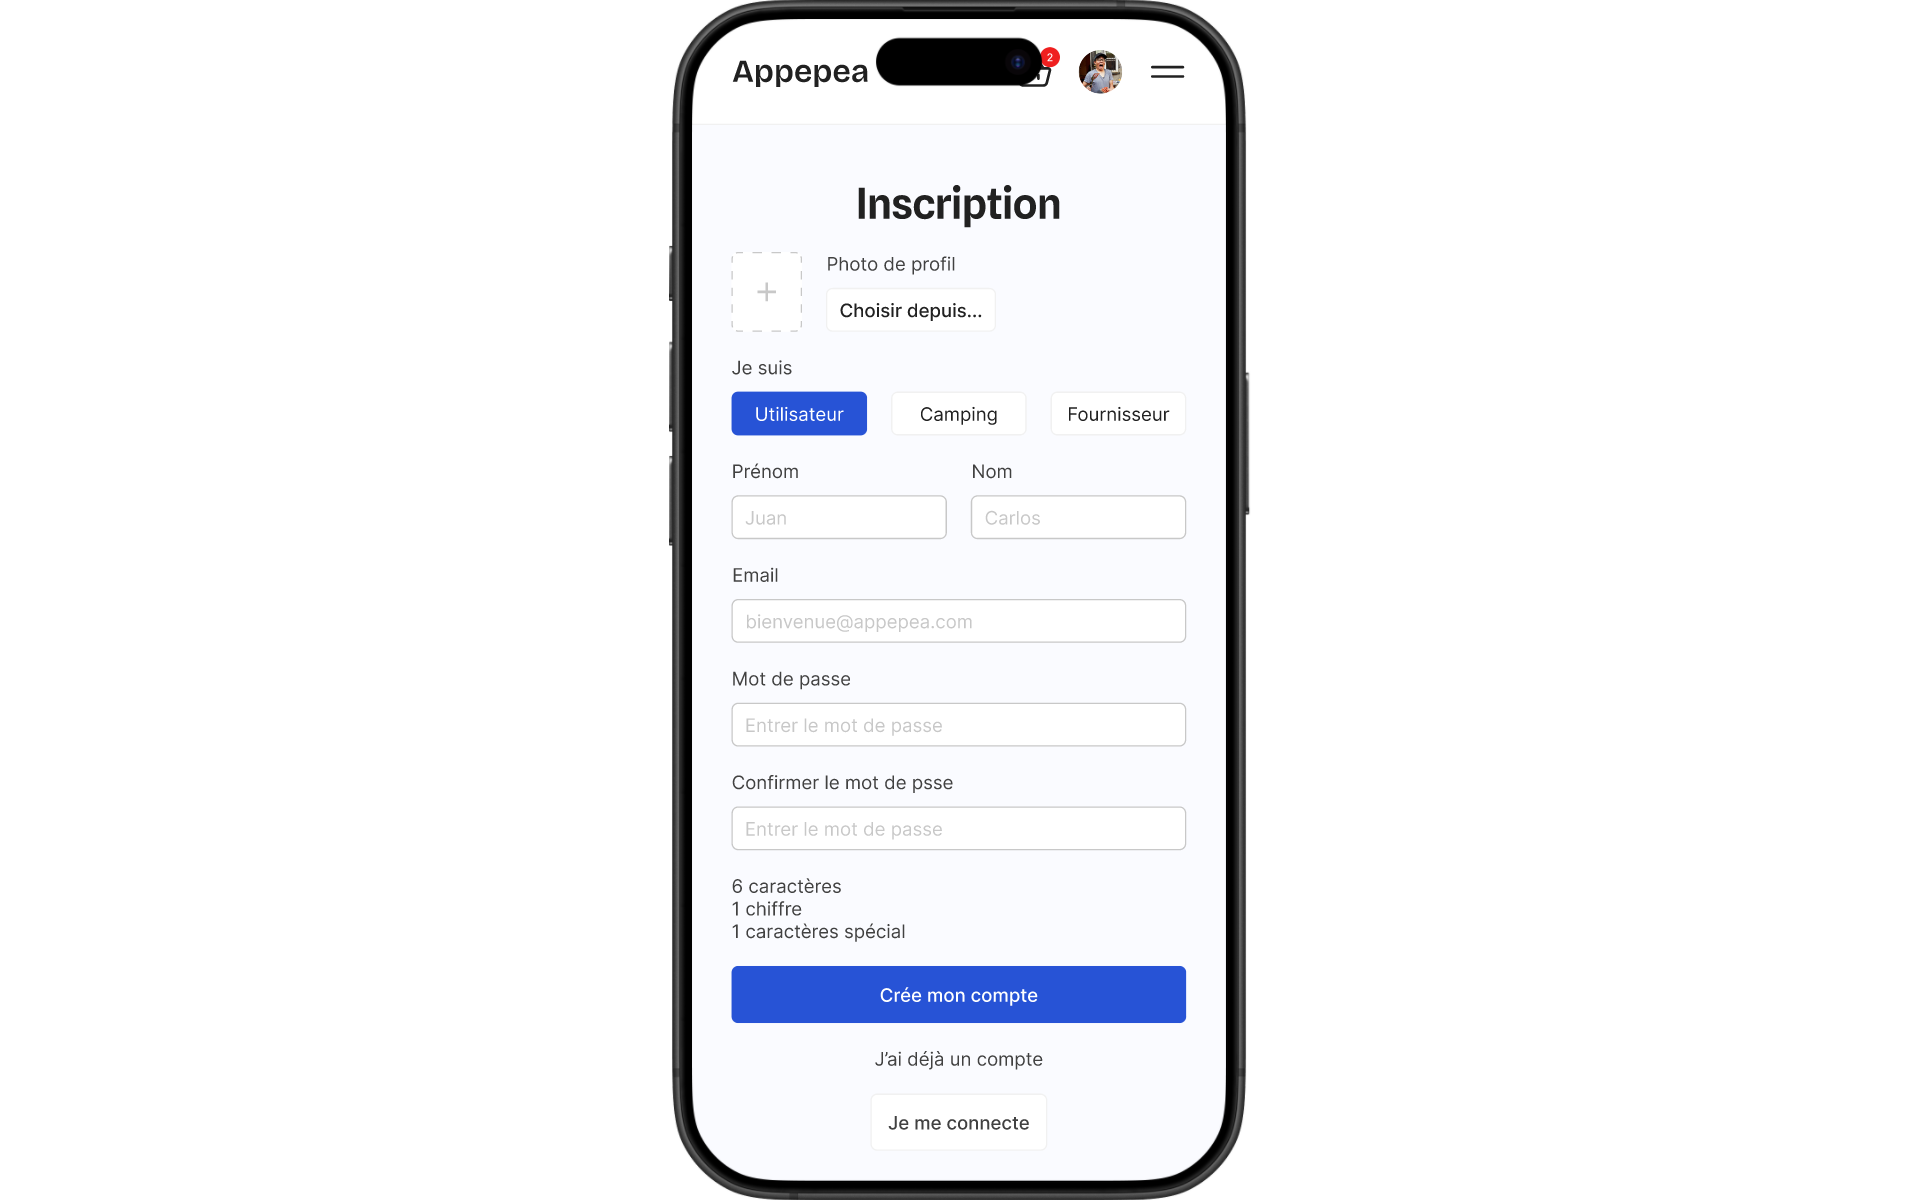
\includegraphics[height=5.5cm]{../img/maquette/inscription.png}
				\caption{	
					\centering			
  					\href{https://github.com/Matteo-K/Soutenance_E-delic/blob/main/img/maquette/inscription.png}{\underline{Inscription Utilisateur}}.\\
  					\textit{Source : Maquette - Théo Le Gourrierec}
				}
  				\label{fig:inscription}
  			\end{figure}
		}
		
		\only<6> {
			\addtocounter{figure}{1}
			\begin{figure}[t]
  				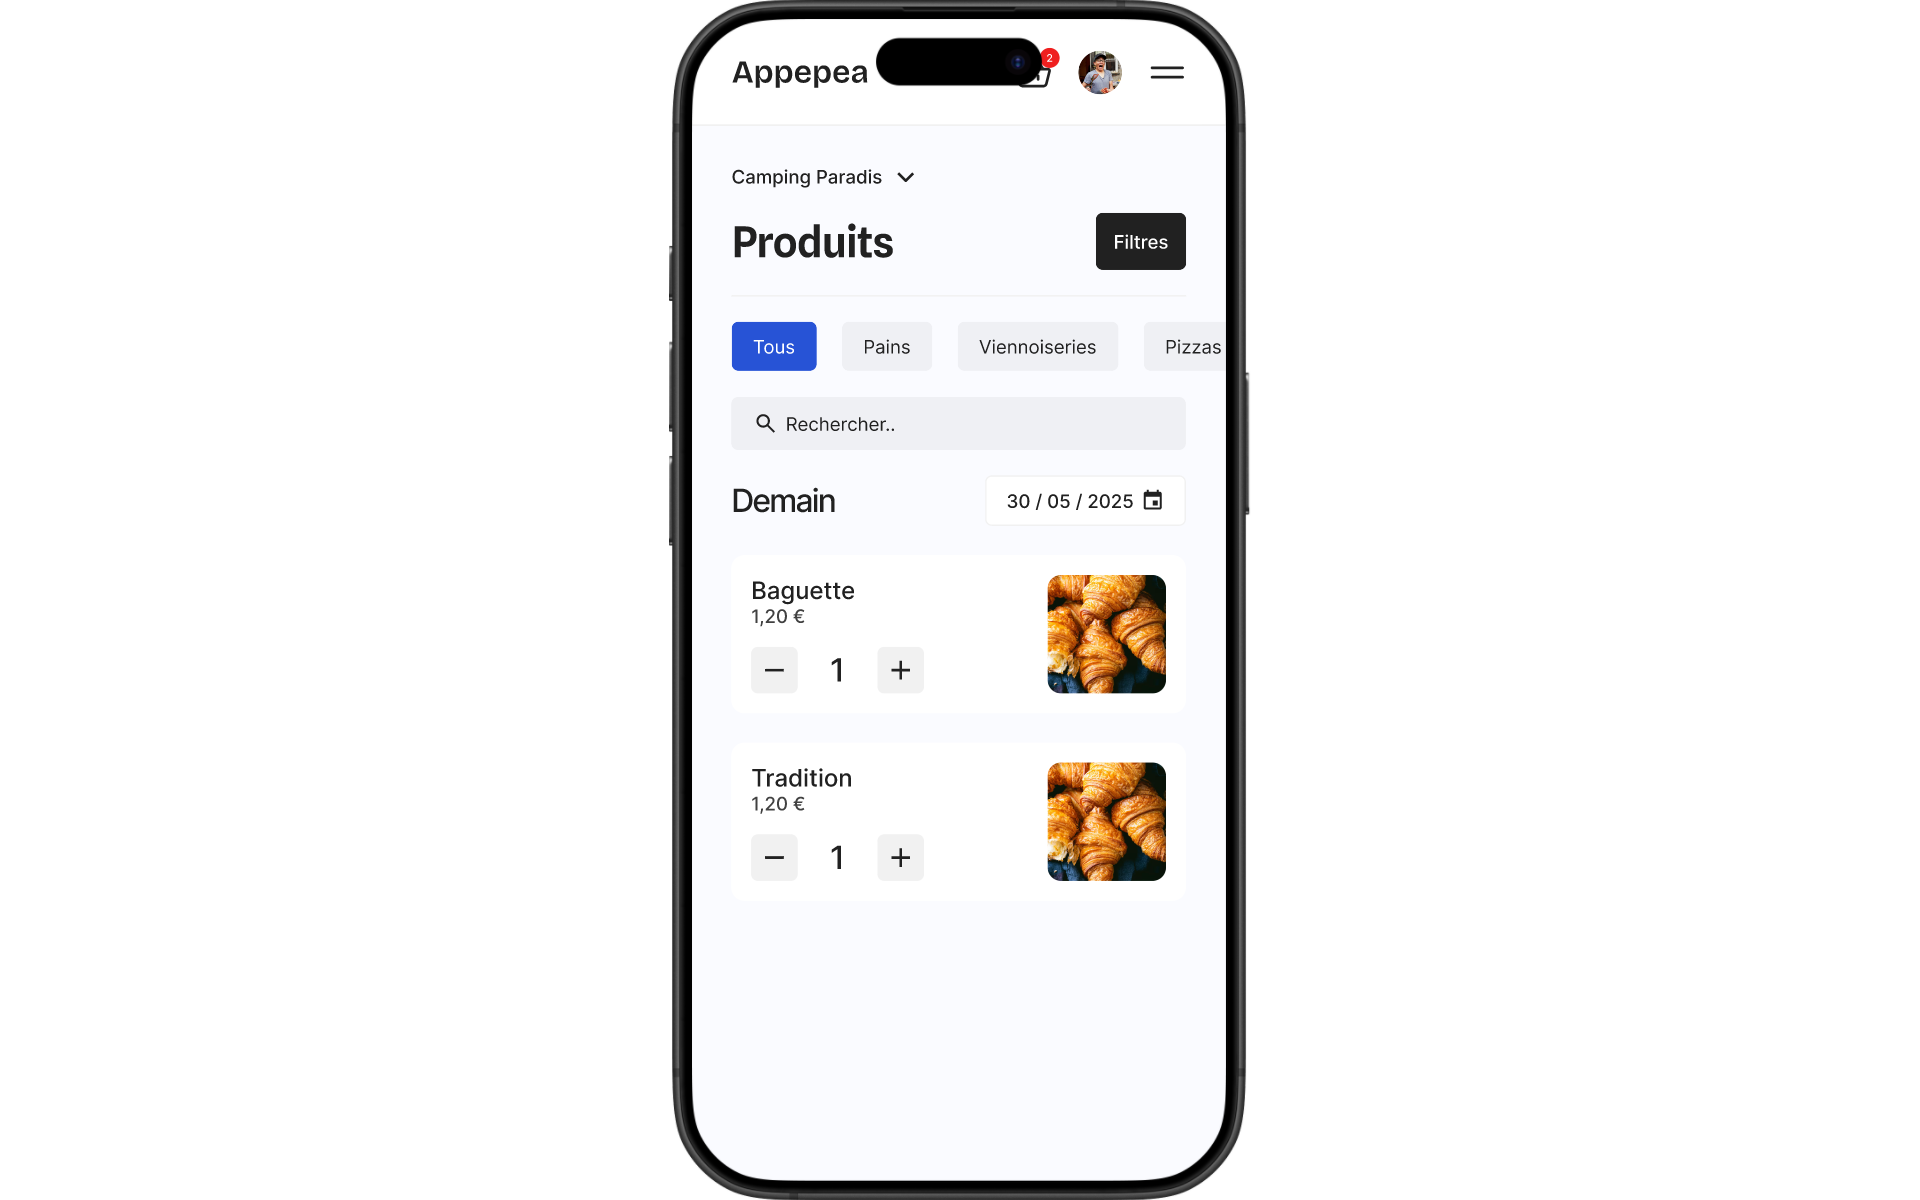
\includegraphics[height=5.5cm]{../img/maquette/controlle_acces_client.png}
				\caption{	
					\centering			
  					\href{https://github.com/Matteo-K/Soutenance_E-delic/blob/main/img/maquette/controlle_acces_client.png}{\underline{Affichage d'un hébergement en tant que \textbf{client}}}.\\
  					\textit{Source : Maquette - Théo Le Gourrierec}
				}
  				\label{fig:controlle_acces_client}
  			\end{figure}
		}
		
		\only<7> {
			\addtocounter{figure}{2}
			\begin{figure}[t]
  				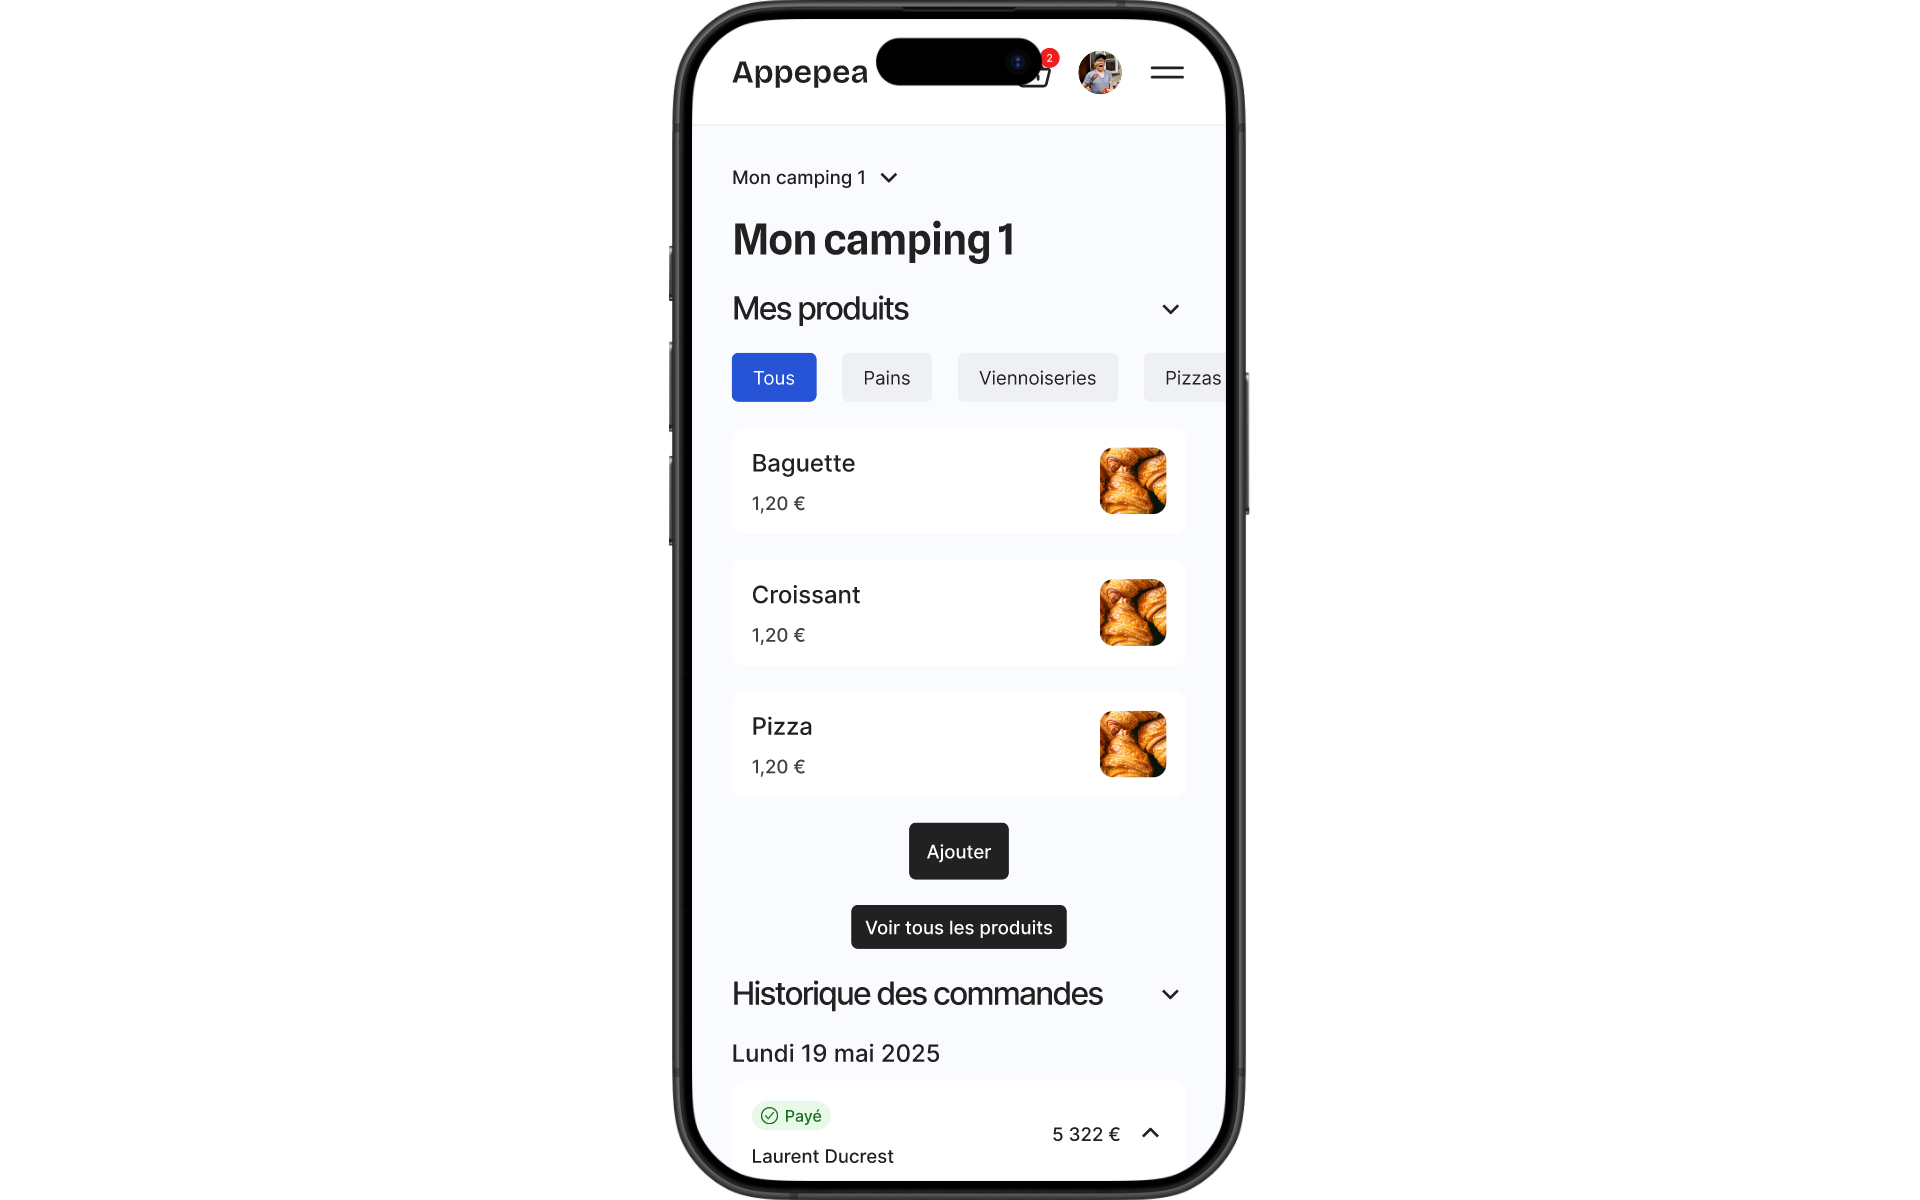
\includegraphics[height=5.5cm]{../img/maquette/controlle_acces_hebergement.png}
				\caption{	
					\centering			
  					\href{https://github.com/Matteo-K/Soutenance_E-delic/blob/main/img/maquette/controlle_acces_hebergement.png}{\underline{Affichage d'un hébergement en tant que \textbf{hébergement}}}.\\
  					\textit{Source : Maquette - Théo Le Gourrierec}
				}
  				\label{fig:controlle_acces_hebergement}
  			\end{figure}
		}
		
		\only<8> {
			\addtocounter{figure}{3}
			\begin{figure}[t]
  				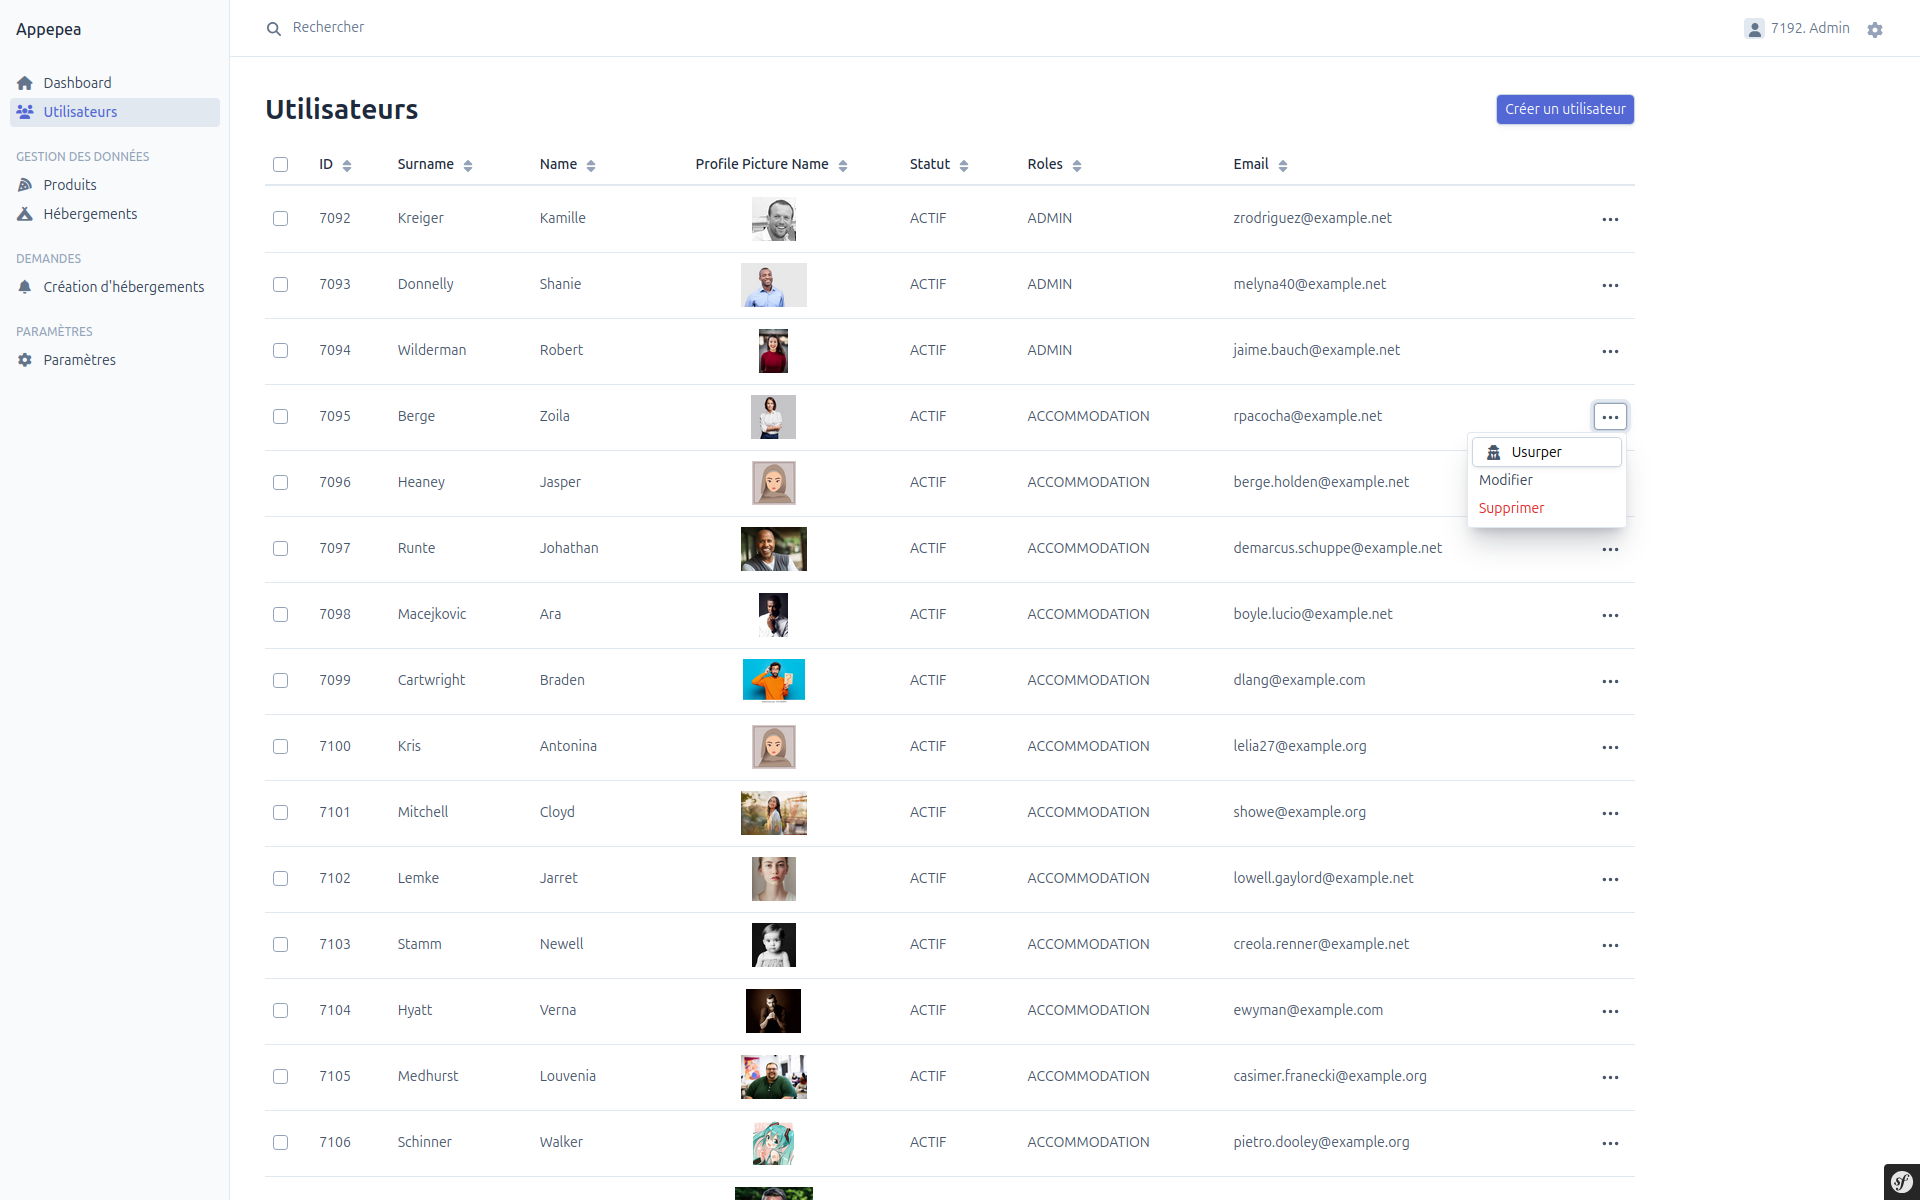
\includegraphics[height=5.5cm]{../img/localhost/usurpation.png}
				\caption{	
					\centering			
  					\href{https://github.com/Matteo-K/Soutenance_E-delic/blob/main/img/localhost/usurpation.png}{\underline{Usurpation d'utilisateur}}.\\
  					\textit{Source : Application - Mattéo Kervadec}
				}
  				\label{fig:usurpation}
  			\end{figure}
		}
  		
	\end{center}
	\vfill
\end{frame}

\begin{frame}{Solutions apportées aux projets}
	\begin{beamercolorbox}[wd=\paperwidth,ht=1.5em,dp=0.5em,leftskip=0.5cm]{section in head/foot}
  		\large \textbf{Réalisation 3 :} \normalsize Développement de la logique métier e-commerce
	\end{beamercolorbox}
	\vspace{0.5em}
	\begin{center}
		\only<1-4> {
  			\begin{minipage}{0.9\textwidth}
  				\textbf{Situation :} Plateforme sans fonctionnalité de commande ou panier. \pause \\
  				\textbf{Tâche :} Sélectionner un produit suivant sa disponibilité. \pause \\
  				\textbf{Action :}
				\begin{itemize}
					\item Gestion des produits
					\item Gestion du panier (API REST)
					\item Implémentation d'un service de disponibilité
				\end{itemize}
				\pause

				\textbf{Résultat :} Création et sélection de produit fluide et dynamique.
  			\end{minipage}
  		}
  		
  		\only<5> {
			\begin{figure}[t]
  				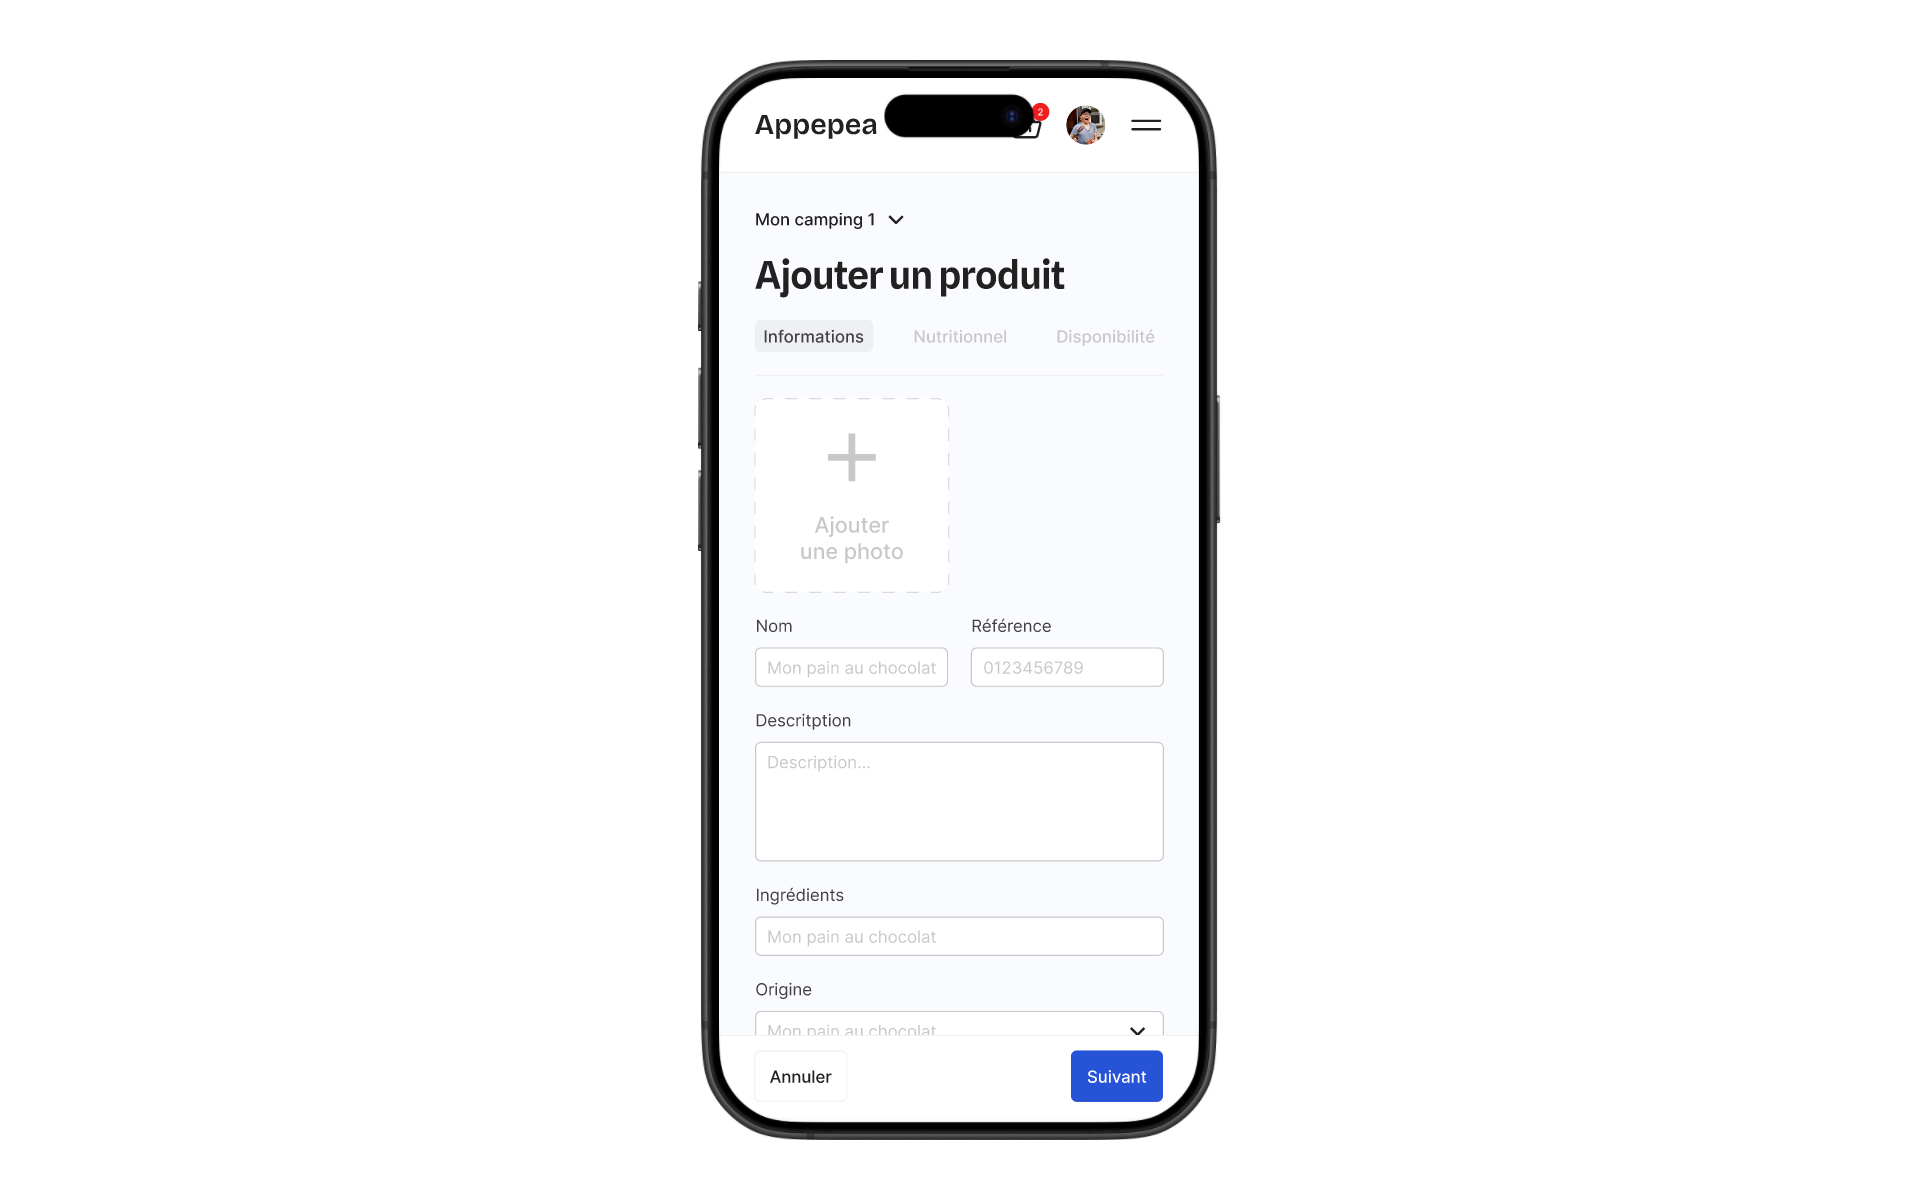
\includegraphics[height=5.5cm]{../img/maquette/crud_produit.png}
				\caption{	
					\centering			
  					\href{https://github.com/Matteo-K/Soutenance_E-delic/blob/main/img/maquette/crud_produit.png}{\underline{Création d'un produit}}.\\
  					\textit{Source : Maquette - Théo Le Gourrierec}
				}
  				\label{fig:crud_produit}
  			\end{figure}
		}
		
		\only<6> {
			\addtocounter{figure}{1}
			\begin{figure}[t]
  				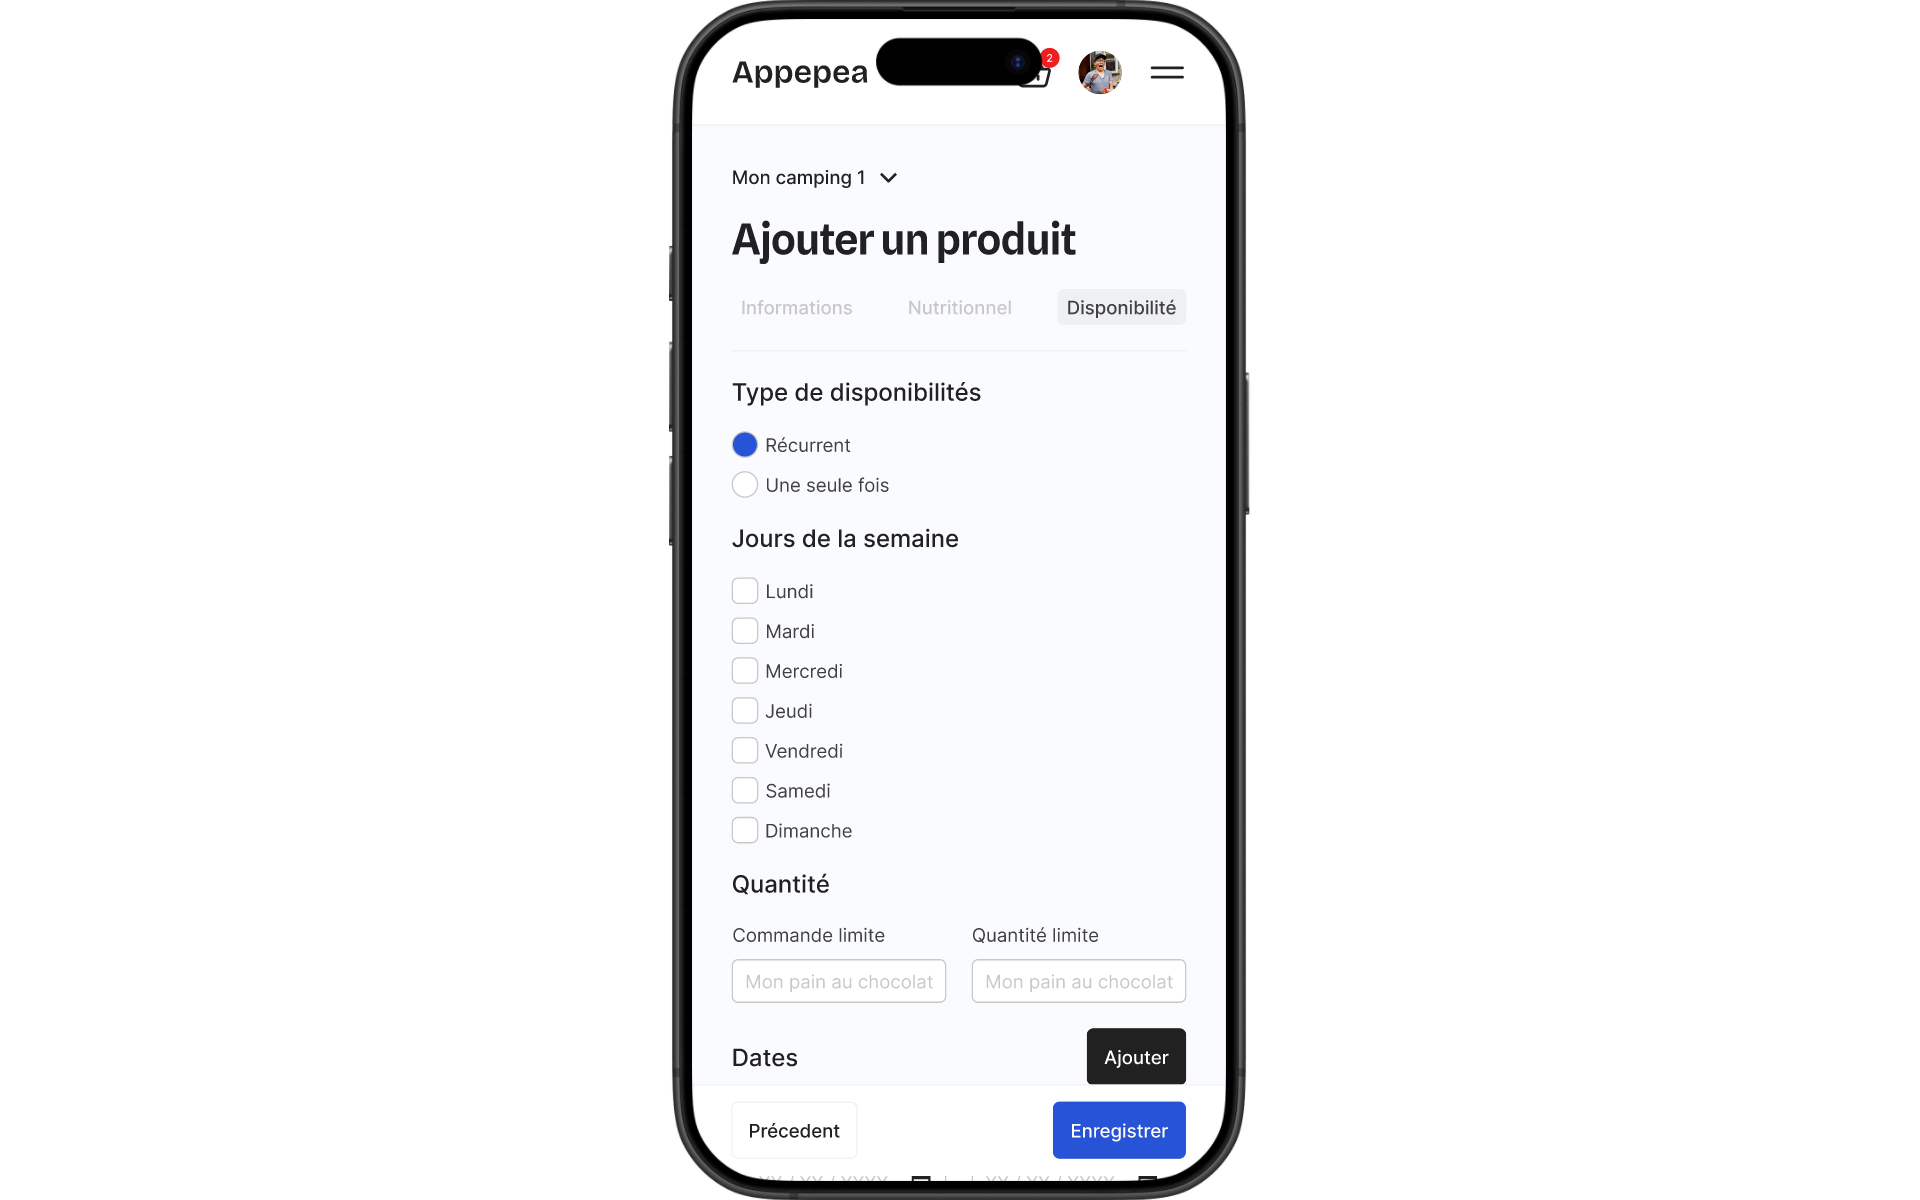
\includegraphics[height=5.5cm]{../img/maquette/disponibilite_produit.png}
				\caption{	
					\centering			
  					\href{https://github.com/Matteo-K/Soutenance_E-delic/blob/main/img/maquette/disponibilite_produit.png}{\underline{Mise en place de la disponibilité}}.\\
  					\textit{Source : Maquette - Théo Le Gourrierec}
				}
  				\label{fig:disponibilite_produit}
  			\end{figure}
		}
		
		\only<7> {
			\addtocounter{figure}{2}
			\begin{figure}[t]
  				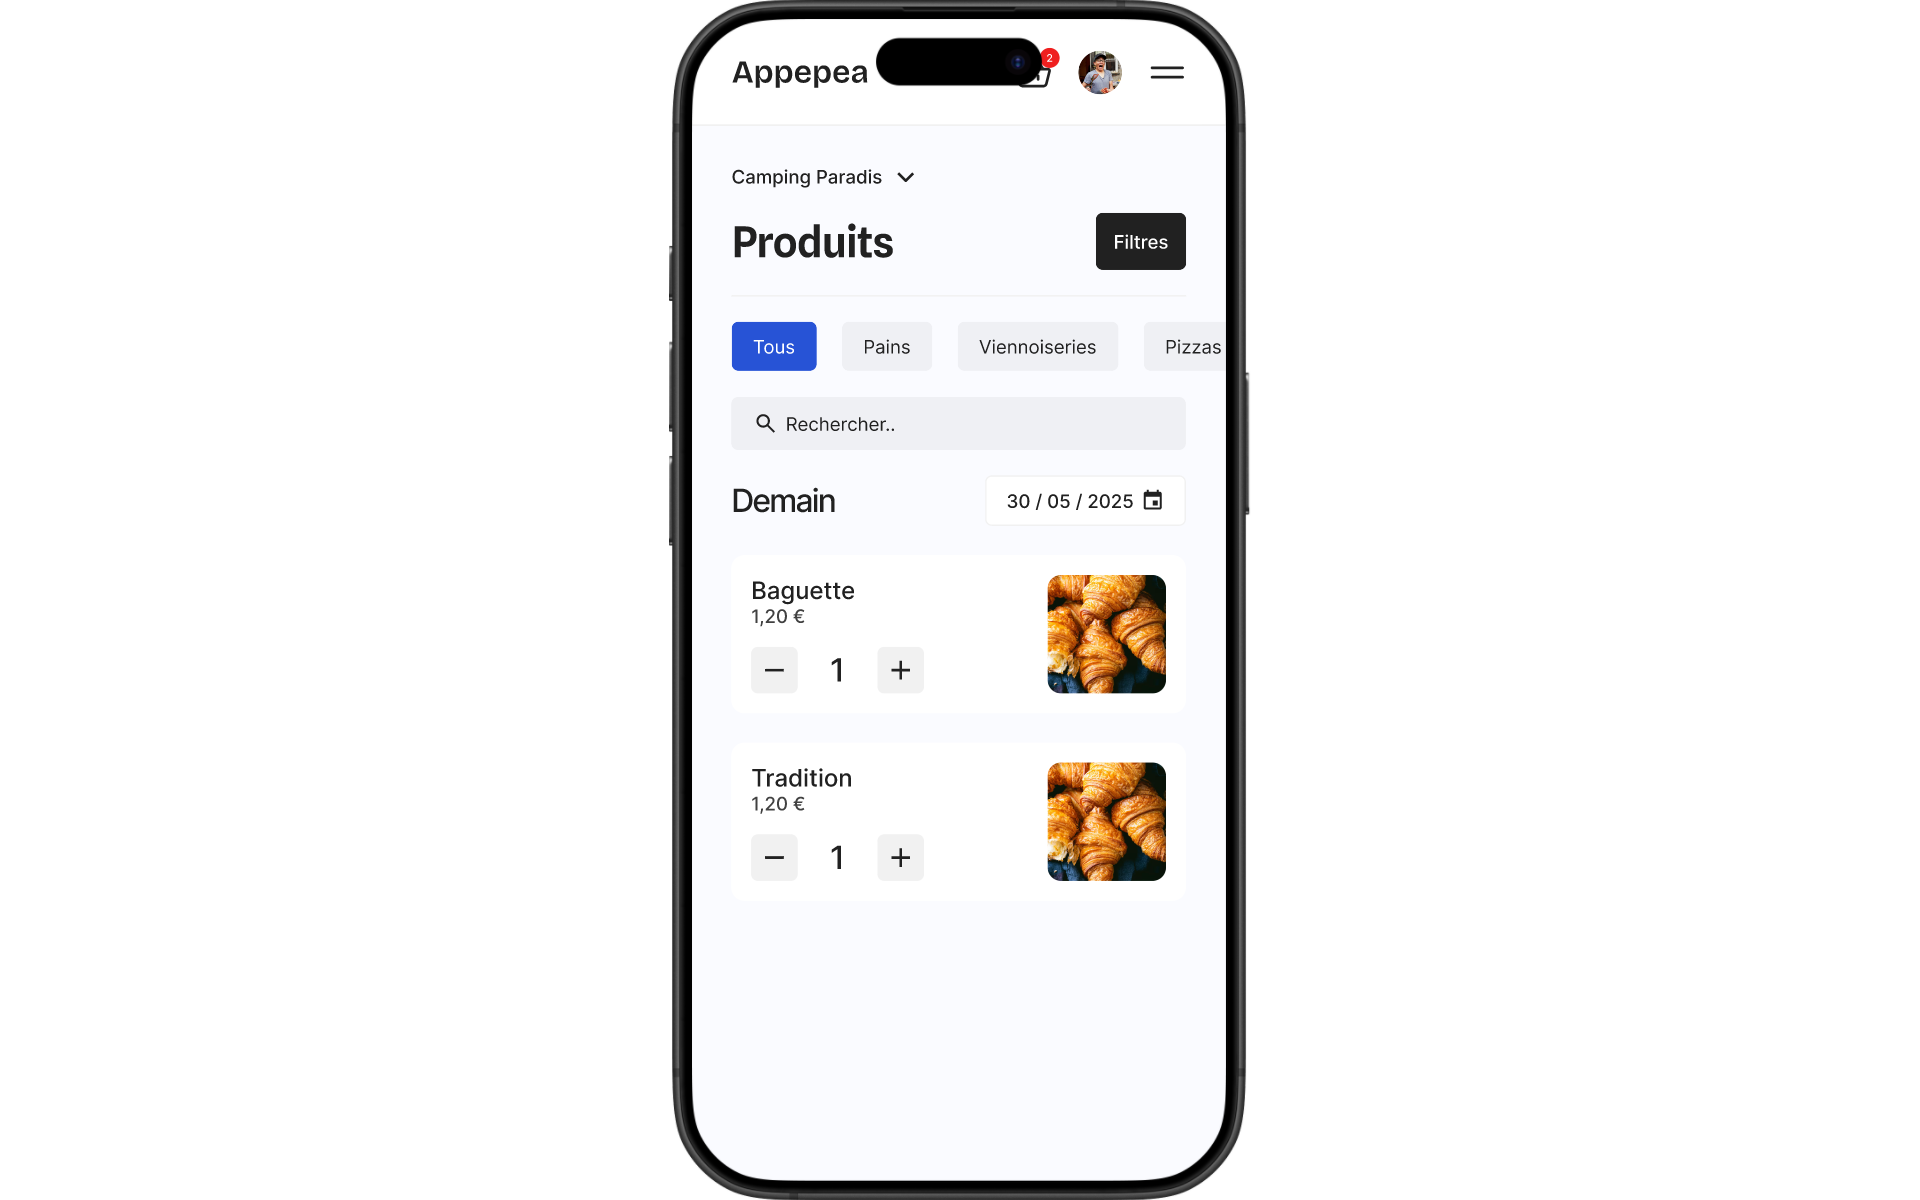
\includegraphics[height=5.5cm]{../img/maquette/controlle_acces_client.png}
				\caption{
					\centering
  					\href{https://github.com/Matteo-K/Soutenance_E-delic/blob/main/img/maquette/controlle_acces_client.png}{\underline{Modification du panier}}.\\
  					\textit{Source : Maquette - Théo Le Gourrierec}
				}
  				\label{fig:modification_panier}
  			\end{figure}
		}
		
		\only<8> {
			\addtocounter{figure}{3}
			\begin{figure}[t]
  				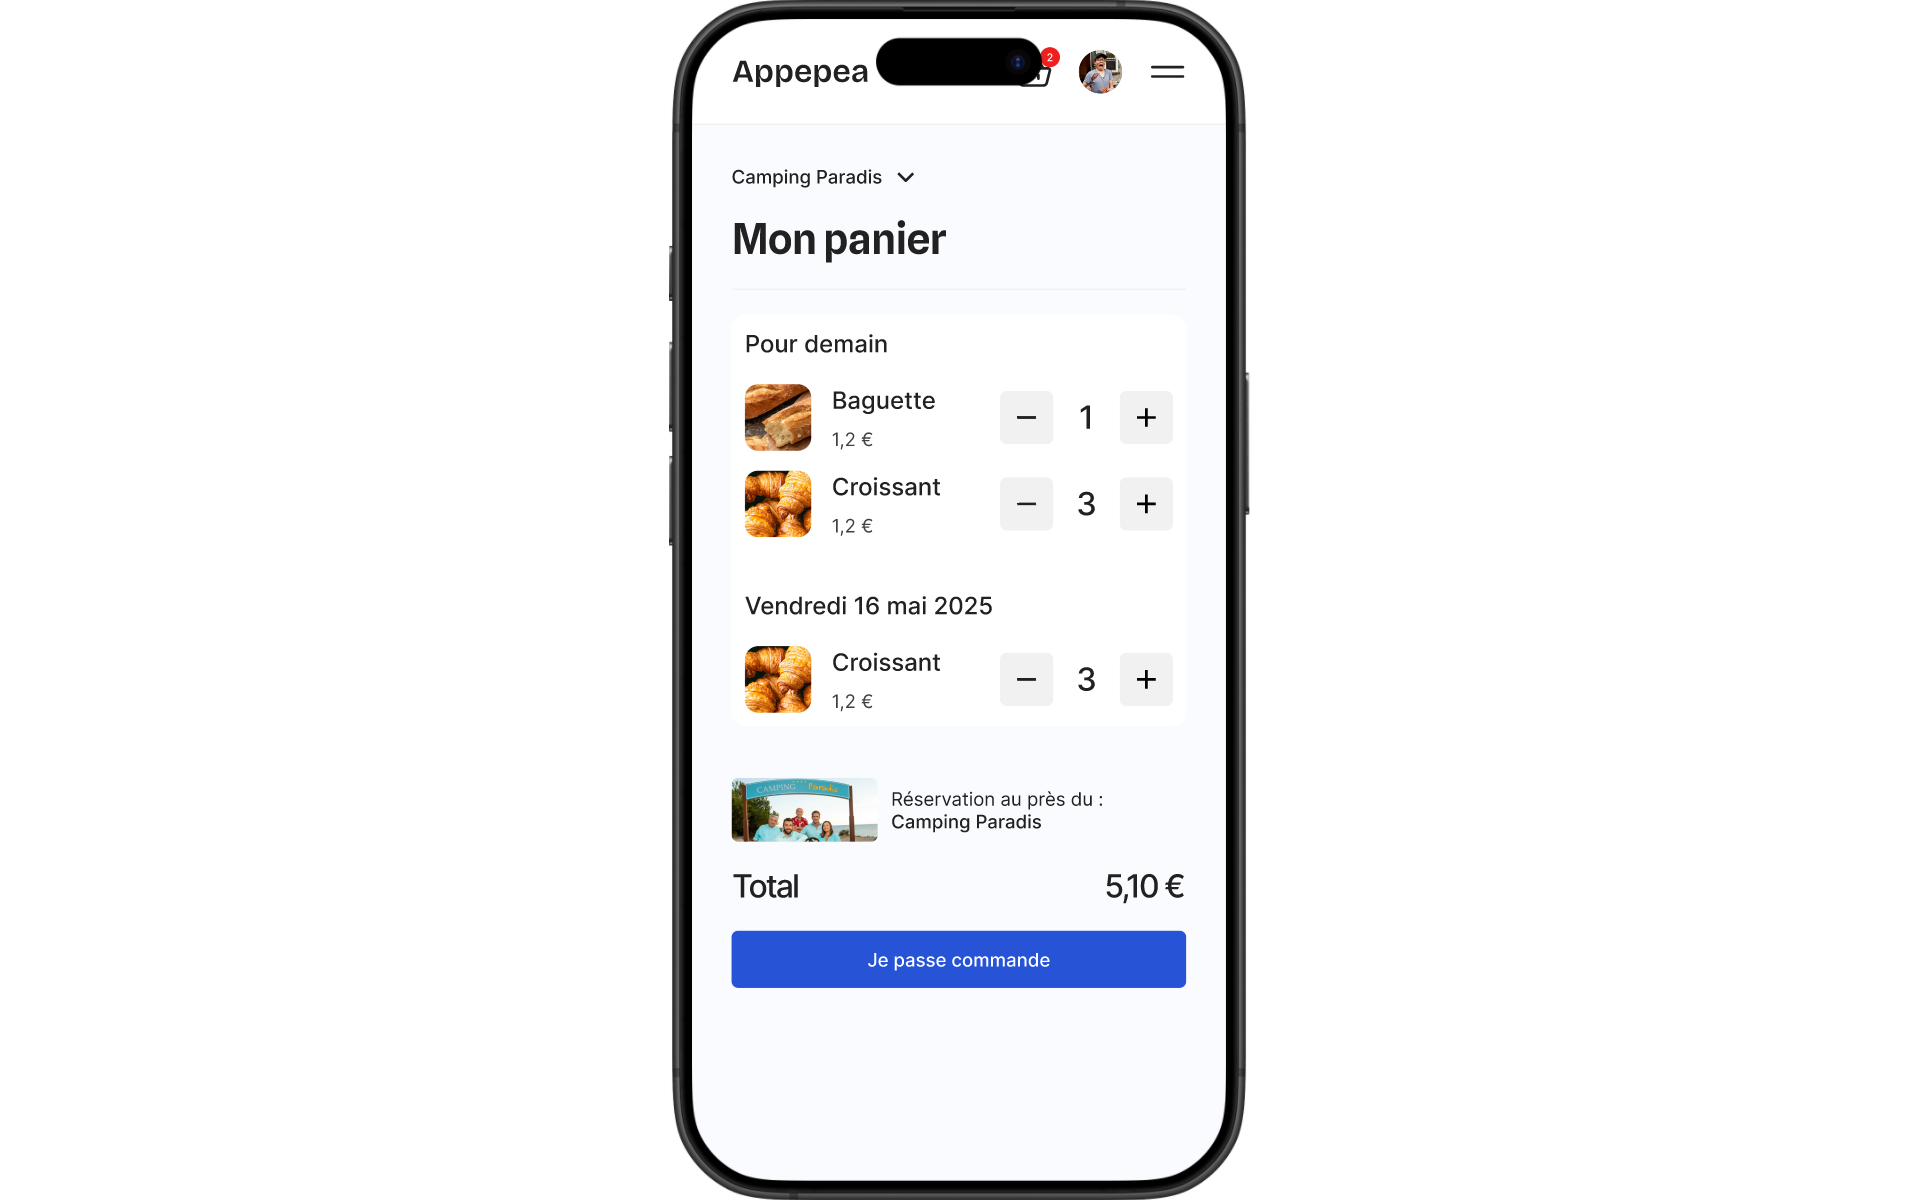
\includegraphics[height=5.5cm]{../img/maquette/panier.png}
				\caption{
					\centering
  					\href{https://github.com/Matteo-K/Soutenance_E-delic/blob/main/img/maquette/panier.png}{\underline{Visualisation du panier}}.\\
  					\textit{Source : Maquette - Théo Le Gourrierec}
				}
  				\label{fig:panier}
  			\end{figure}
		}
	\end{center}
	\vfill
\end{frame}

\begin{frame}{Solutions apportées aux projets}
	\begin{beamercolorbox}[wd=\paperwidth,ht=1.5em,dp=0.5em,leftskip=0.5cm]{section in head/foot}
  		\large \textbf{Réalisation 4 :} \normalsize Mise en place de la procédure de paiement et réservation
	\end{beamercolorbox}
	\vspace{0.5em}
	\begin{center}
		\only<1-4> {	
	  		\begin{minipage}{0.9\textwidth}
  				\textbf{Situation :} Conclure la procédure de gestion. \pause \\
  				\textbf{Tâche :} Volonté d'encaisser et retracer les commandes. \pause \\
  				\textbf{Action :}
  				\begin{itemize}
  					\item Integration de stripe pour les paiements sécurisés
  					\item Mise en place d'historique de commande
  				\end{itemize}
  				\pause
  				
				\textbf{Résultat :} Traçage et méthode de paiement fonctionnel qui nécessiterait des améliorations.
				\begin{itemize}
					\item Porte-monnaie virtuelle
					\item Gestion de suivi de livraison
				\end{itemize}
  			\end{minipage}
  		}
  		
  		\only<5> {
			\begin{figure}[t]
  				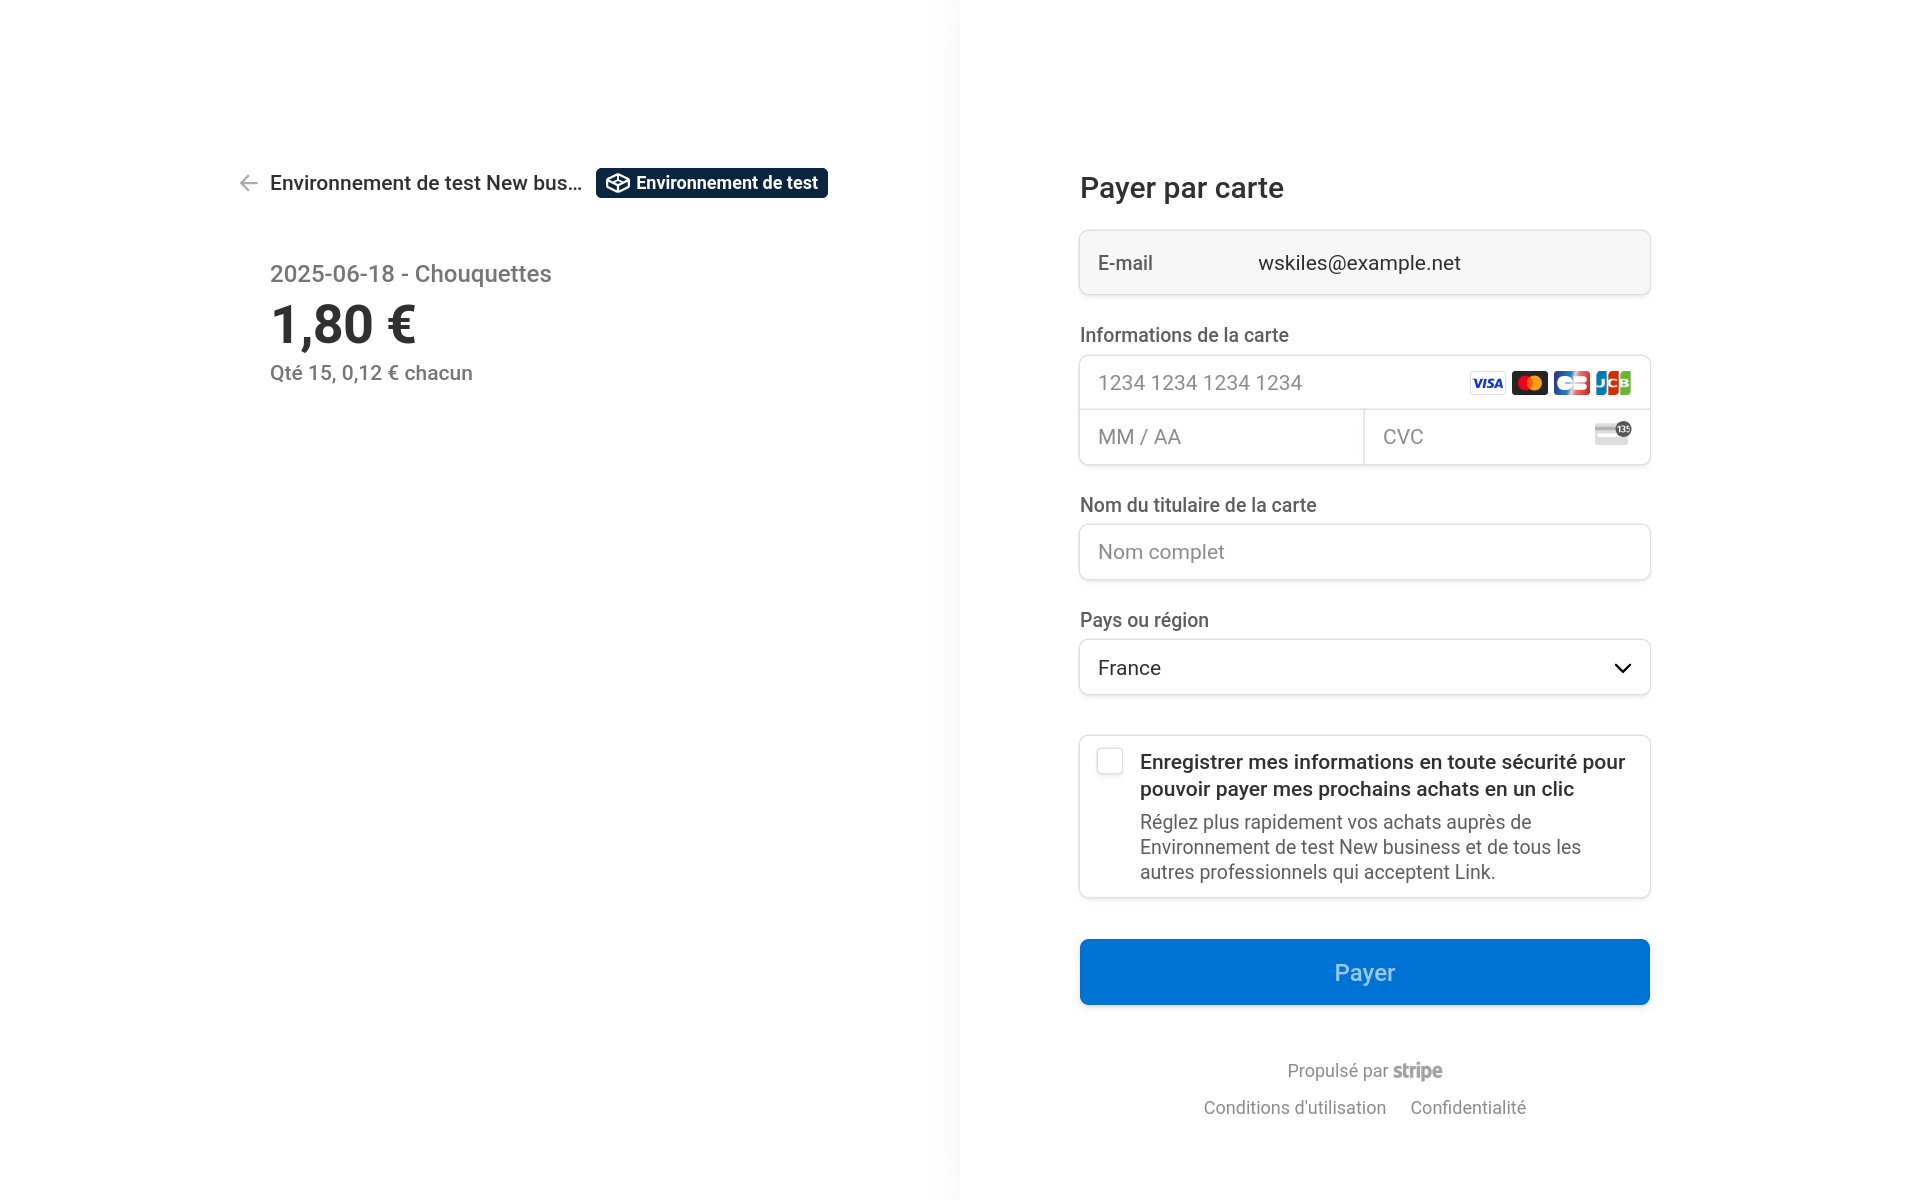
\includegraphics[height=5.5cm]{../img/localhost/stripe.png}
				\caption{	
					\centering			
  					\href{https://github.com/Matteo-K/Soutenance_E-delic/blob/main/img/maquette/crud_produit.png}{\underline{Paiement par stripe}}.\\
  					\textit{Source : Application - Mattéo Kervadec}
				}
  				\label{fig:stripe}
  			\end{figure}
		}
		
		\only<6> {
			\addtocounter{figure}{1}
			\begin{figure}[t]
  				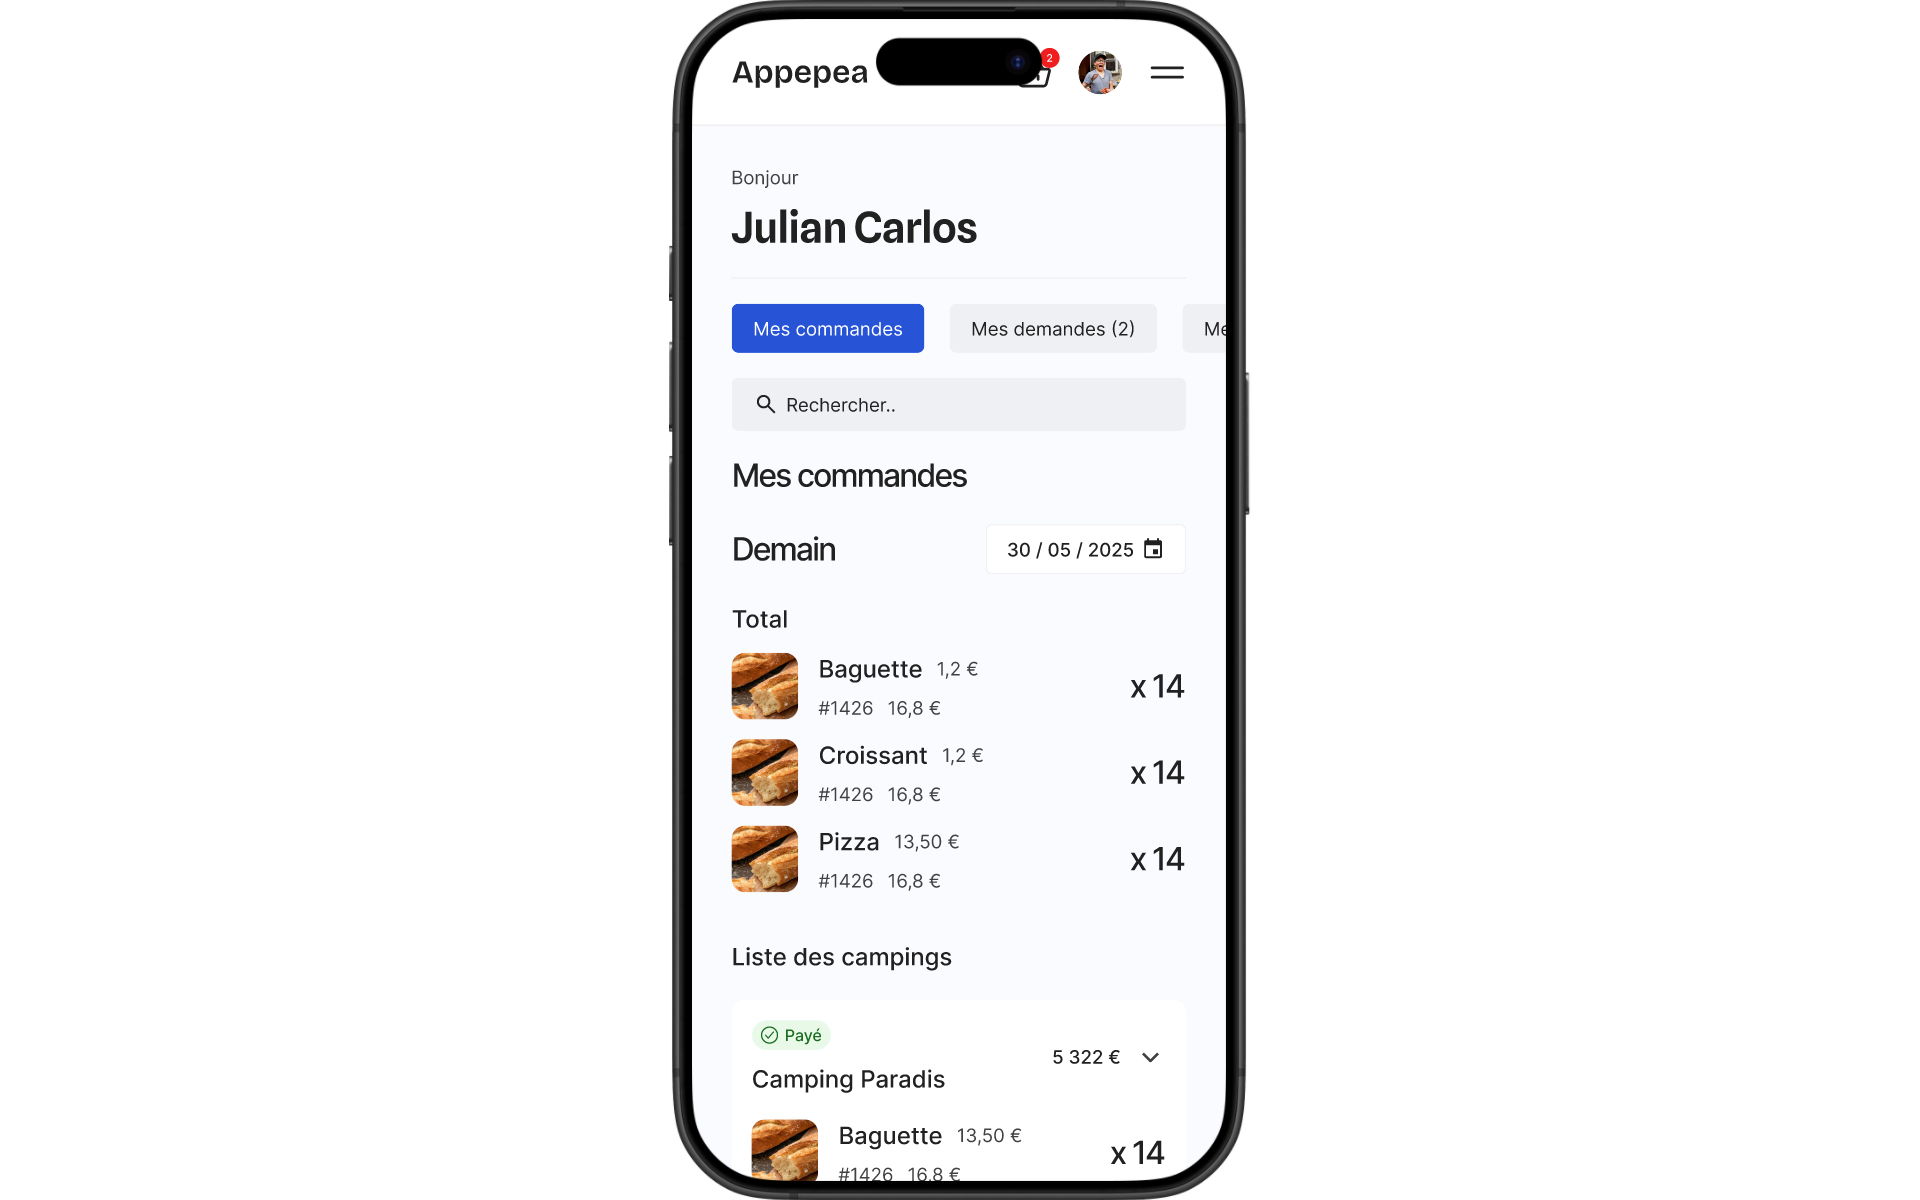
\includegraphics[height=5.5cm]{../img/maquette/historique_commande.png}
				\caption{	
					\centering
  					\href{https://github.com/Matteo-K/Soutenance_E-delic/blob/main/img/maquette/historique_commande.png}{\underline{Historique des commandes}}.\\
  					\textit{Source : Maquette - Théo Le Gourrierec}
				}
  				\label{fig:disponibilite_produit}
  			\end{figure}
		}
	\end{center}
	\vfill
\end{frame}

\planSlide{5}

% === CONCLUSION ===
\begin{frame}[label=conclusion]{Conclusion}
  	\begin{beamercolorbox}[wd=\paperwidth,ht=1.5em,dp=0.5em,leftskip=0.5cm]{section in head/foot}
  		\large \textbf{Bilan de la situation}
	\end{beamercolorbox}
	\vspace{0.5em}
	\begin{center}
  		\begin{minipage}{0.9\textwidth}
	  		Objectifs atteints, quelques améliorations possibles.
  			\begin{itemize}
  				\item Application de e-commerce fonctionnelle
			  	\item Interface graphique à finaliser
			  	\item Fonctionnalités essentielles sont implémentés
			  	\item Pistes de fonctionnalité à ajouter : 
			  	\begin{itemize}
			  		\item Porte-monnaie
			  		\item Gestion d'abonnement
			  	\end{itemize}
			\end{itemize}
  		\end{minipage}
	\end{center}
	\vfill
\end{frame}

\begin{frame}{Conclusion}
  	\begin{beamercolorbox}[wd=\paperwidth,ht=1.5em,dp=0.5em,leftskip=0.5cm]{section in head/foot}
  		\large \textbf{Bilan technique}
	\end{beamercolorbox}
	\vspace{0.5em}
	\begin{center}
  		\begin{minipage}{0.9\textwidth}
  			\begin{itemize}
  				\item \faLaptopCode\ Mise en place d'une architecture MVC
  				\item \faCodeBranch\ Découverte et maitrise du framework backend \textbf{Symfony}
  				\item \faLock\ Gestion d'utilisateur et de sécurité des routes
  				\item \faBolt\ Interactions sans rechargement via \textbf{Turbo/Stimulus}
  				\item \faDatabase\ Structuration et modélisation de base de données
			\end{itemize}
  		\end{minipage}
	\end{center}
	\vfill
\end{frame}

\begin{frame}{Conclusion}
  	\begin{beamercolorbox}[wd=\paperwidth,ht=1.5em,dp=0.5em,leftskip=0.5cm]{section in head/foot}
  		\large \textbf{Bilan humain}
	\end{beamercolorbox}
	\vspace{0.5em}
	\begin{center}
  		\begin{minipage}{1\textwidth}
  			\textbf{\faCheck\ Fier du travail produit}
  			\begin{itemize}
  				\item Progression en autonomie
  				\item Amélioration de la prise de décision
  				\item Acceptation de la suppression de certaines fonctionnalités
  				\item Communication directe et feedback régulier
  				\item Satisfaction de la réalisation finale
  			\end{itemize}
  				
  			\pause

  			\textbf{\faTimes\ Déçu de certains points}
  			\begin{itemize}
  				\item Manque d'outis de gestion
		  		\item Impression de stagnation de productivité
  			\end{itemize}
  		\end{minipage}
	\end{center}
	\vfill
\end{frame}

\begin{frame}[label=remerciements]{\Large Remerciements}
    \logoEdeclic
    \begin{center}
        \vspace{1em}
        \begin{minipage}{0.9\textwidth}
        		Un grand merci à toute l'équipe de \textbf{e-declic} et mon tuteur de stage \textbf{M. Morvant Michel} pour l'accueil et leurs accompagnements durant ce stage. \vspace{0.25cm} \\
            Merci à l'\textbf{IUT de Lannion} pour m'avoir offert cette opportunité de formation. \vspace{0.25cm} \\
            Je remercie également \textbf{le jury} pour le temps accordé et l'intérêt porté à mon travail. \vspace{0.25cm} \\
            Enfin, je suis heureux de pouvoir poursuivre cette expérience chez \textbf{e-declic} en \textbf{alternance dès cet été}.
        \end{minipage}
    \end{center}
    \vfill
\end{frame}

\begin{frame}[label=sources]{Sources}
	\begin{itemize}
		\item \href{https://www.e-declic.com/}{\underline{Site web E-declic}}
		\item \href{https://www.francenum.gouv.fr/activateurs/e-declic}{\underline{FranceNum - Caractéristiques E-declic}}
		\item \href{https://annuaire-entreprises.data.gouv.fr/entreprise/e-declic-453413296}{\underline{Annuaire des entreprises - Caractéristiques E-declic}}
		\item \href{https://entreprises.lefigaro.fr/e-declic-56/entreprise-453413296}{\underline{lefigaro entreprise - Caractéristiques E-declic}}
		\item \href{https://github.com/Matteo-K/Soutenance_E-delic/tree/main/img}{\underline{Ressources de la soutenance}}
	\end{itemize}
	\vfill
\end{frame}

\end{document}